%  LaTeX support: latex@mdpi.com 
%  For support, please attach all files needed for compiling as well as the log file, and specify your operating system, LaTeX version, and LaTeX editor.

%=================================================================
\documentclass[ijms,article,accept,moreauthors,pdftex]{Definitions/mdpi}
%\usepackage[table,xcdraw]{xcolor}

\usepackage{xcolor}
\usepackage{soul}

% For posting an early version of this manuscript as a preprint, you may use "preprints" as the journal and change "submit" to "accept". The document class line would be, e.g., \documentclass[preprints,article,accept,moreauthors,pdftex]{mdpi}. This is especially recommended for submission to arXiv, where line numbers should be removed before posting. For preprints.org, the editorial staff will make this change immediately prior to posting.

%--------------------
% Class Options:
%--------------------
%----------
% journal
%----------
% Choose between the following MDPI journals:
% ijms

%---------
% article
%---------
% The default type of manuscript is "article", but can be replaced by: 
% abstract, addendum, article, book, bookreview, briefreport, casereport, comment, commentary, communication, conferenceproceedings, correction, conferencereport, entry, expressionofconcern, extendedabstract, datadescriptor, editorial, essay, erratum, hypothesis, interestingimage, obituary, opinion, projectreport, reply, retraction, review, perspective, protocol, shortnote, studyprotocol, systematicreview, supfile, technicalnote, viewpoint, guidelines, registeredreport, tutorial
% supfile = supplementary materials

%----------
% submit
%----------
% The class option "submit" will be changed to "accept" by the Editorial Office when the paper is accepted. This will only make changes to the frontpage (e.g., the logo of the journal will get visible), the headings, and the copyright information. Also, line numbering will be removed. Journal info and pagination for accepted papers will also be assigned by the Editorial Office.

%------------------
% moreauthors
%------------------
% If there is only one author the class option oneauthor should be used. Otherwise use the class option moreauthors.

%---------
% pdftex
%---------
% The option pdftex is for use with pdfLaTeX. If eps figures are used, remove the option pdftex and use LaTeX and dvi2pdf.

%=================================================================
% MDPI internal commands
\firstpage{1} 
\makeatletter 
\setcounter{page}{\@firstpage} 
\makeatother
\pubvolume{1}
\issuenum{1}
\articlenumber{0}
\pubyear{2021}
\copyrightyear{2021}
\externaleditor{Academic Editor: \hl{Firstname Lastname} %MDPI: please add this if available.
} % For journal Automation, please change Academic Editor to "Communicated by"
\datereceived{} 
\dateaccepted{} 
\datepublished{} 
\hreflink{https://doi.org/} % If needed use \linebreak
%------------------------------------------------------------------
% The following line should be uncommented if the LaTeX file is uploaded to arXiv.org
%\pdfoutput=1

%=================================================================
% Add packages and commands here. The following packages are loaded in our class file: fontenc, inputenc, calc, indentfirst, fancyhdr, graphicx, epstopdf, lastpage, ifthen, lineno, float, amsmath, setspace, enumitem, mathpazo, booktabs, titlesec, etoolbox, tabto, xcolor, soul, multirow, microtype, tikz, totcount, changepage, paracol, attrib, upgreek, cleveref, amsthm, hyphenat, natbib, hyperref, footmisc, url, geometry, newfloat, caption

%=================================================================
%% Please use the following mathematics environments: Theorem, Lemma, Corollary, Proposition, Characterization, Property, Problem, Example, ExamplesandDefinitions, Hypothesis, Remark, Definition, Notation, Assumption
%% For proofs, please use the proof environment (the amsthm package is loaded by the MDPI class).

%=================================================================
% Full title of the paper (Capitalized)
\Title{Investigating the Molecular Processes Behind the Cell-Specific Toxicity Response to Titanium Dioxide Nanobelts}

% MDPI internal command: Title for citation in the left column
\TitleCitation{Investigating the Molecular Processes Behind the Cell-Specific Toxicity Response to Titanium Dioxide Nanobelts}

% Author Orchid ID: enter ID or remove command
\newcommand{\orcidauthorA}{0000-0002-9454-4783} % Add \orcidA{} behind the author's name
\newcommand{\orcidauthorB}{0000-0002-5301-3142} % Add \orcidB{} behind the author's name
\newcommand{\orcidauthorC}{0000-0001-7542-0286} % Add \orcidC{} behind the author's name
\newcommand{\orcidauthorD}{0000-0002-7699-8191} % Add \orcidD{} behind the author's name

% Authors, for the paper (add full first names)
\Author{\hl{Laurent A. Winckers} %MDPI: Please carefully check the accuracy of names and affiliations.
 $^{1}$\orcidA{}, Chris \hl{T.} %MDPI: we added dot for middle name abbreviation, please confirm. Correct.
 Evelo $^{1,2}$\orcidB{}, Egon \hl{L.} Willighagen $^{1}$\orcidC{} and Martina Kutmon $^{1,2,}$*\orcidD{}}

% MDPI internal command: Authors, for metadata in PDF
\AuthorNames{Laurent A Winckers, Chris T Evelo, Egon L Willighagen and Martina Kutmon}

% MDPI internal command: Authors, for citation in the left column
\AuthorCitation{Winckers, L.A.; Evelo, C.T.; Willighagen, E.L.; Kutmon, M.}
% If this is a Chicago style journal: Lastname, Firstname, Firstname Lastname, and Firstname Lastname.

% Affiliations / Addresses (Add [1] after \address if there is only one affiliation.)
\address{%
$^{1}$ \quad Department of Bioinformatics\hl{---}%MDPI: changed from hyphen into em dash.
BiGCaT, NUTRIM School of Nutrition and Translational Research in Metabolism, Maastricht \hl{University}, Maastricht, NL-6200 MD, The Netherlands; %MDPI: PLEASE add city, state abbreviation postcode, country.
%Reply: Added city, postcode and country.
 \hl{laurent.winckers@maastrichtuniversity.nl (L.A.W.); chris.evelo@maastrichtuniversity.nl (C.T.E.);  egon.willighagen@maastrichtuniversity.nl (E.L.W.)} %MDPI: Newly added information, please confirm.
%Reply: looks good
\\
$^{2}$ \quad Maastricht Centre for Systems Biology (MaCSBio), Maastricht \hl{University}, Maastricht, NL-6200 MD, The Netherlands}
%Reply: Added city, postcode and country.

% Contact information of the corresponding author
\corres{Correspondence: martina.kutmon@maastrichtuniversity.nl}

% Current address and/or shared authorship
%\firstnote{Current address: Affiliation 3} 
%\secondnote{These authors contributed equally to this work.}
% The commands \thirdnote{} till \eighthnote{} are available for further notes

%\simplesumm{} % Simple summary

%\conference{} % An extended version of a conference paper

% Abstract (Do not insert blank lines, i.e. \\) 
\abstract{Some engineered nanomaterials incite toxicological effects, but the underlying molecular processes are understudied. The varied physicochemical properties cause different initial molecular interactions, complicating toxicological predictions. Gene expression data allow us to study the responses of genes and biological processes. Overrepresentation analysis identifies enriched biological processes using the experimental data but prompts broad results instead of detailed toxicological processes. We demonstrate a targeted filtering approach to compare public gene expression data for low and high exposure on three cell lines to titanium dioxide nanobelts. Our workflow finds cell and concentration-specific changes in affected pathways linked to four Gene Ontology terms (apoptosis, inflammation, DNA damage, and oxidative stress) to select pathways with a clear toxicity focus. 
We saw more differentially expressed genes at higher exposure, but our analysis identifies clear differences between the cell lines in affected processes. Colorectal adenocarcinoma cells showed resilience to both concentrations. Small airway epithelial cells displayed a cytotoxic response to the high concentration, but not as strongly as monocytic-like cells. The pathway-gene networks highlighted the gene overlap between altered toxicity-related pathways. The automated workflow is flexible and can focus on other biological processes by selecting other GO terms.}

% Keywords
\keyword{nanomaterials; titanium dioxide; nanobelts; overrepresentation analysis; Gene Ontology; THP1; SAE; Caco-2/HT29-MTX}

% The fields PACS, MSC, and JEL may be left empty or commented out if not applicable
%\PACS{J0101}
%\MSC{}
%\JEL{}

%%%%%%%%%%%%%%%%%%%%%%%%%%%%%%%%%%%%%%%%%%
% Only for the journal Diversity
%\LSID{\url{http://}}

%%%%%%%%%%%%%%%%%%%%%%%%%%%%%%%%%%%%%%%%%%
% Only for the journal Applied Sciences:
%\featuredapplication{Authors are encouraged to provide a concise description of the specific application or a potential application of the work. This section is not mandatory.}
%%%%%%%%%%%%%%%%%%%%%%%%%%%%%%%%%%%%%%%%%%

%%%%%%%%%%%%%%%%%%%%%%%%%%%%%%%%%%%%%%%%%%
% Only for the journal Data:
%\dataset{DOI number or link to the deposited data set in cases where the data set is published or set to be published separately. If the data set is submitted and will be published as a supplement to this paper in the journal Data, this field will be filled by the editors of the journal. In this case, please make sure to submit the data set as a supplement when entering your manuscript into our manuscript editorial system.}

%\datasetlicense{license under which the data set is made available (CC0, CC-BY, CC-BY-SA, CC-BY-NC, etc.)}

%%%%%%%%%%%%%%%%%%%%%%%%%%%%%%%%%%%%%%%%%%
% Only for the journal Toxins
%\keycontribution{The breakthroughs or highlights of the manuscript. Authors can write one or two sentences to describe the most important part of the paper.}

%%%%%%%%%%%%%%%%%%%%%%%%%%%%%%%%%%%%%%%%%%
% Only for the journal Encyclopedia
%\encyclopediadef{Instead of the abstract}
%\entrylink{The Link to this entry published on the encyclopedia platform.}
%%%%%%%%%%%%%%%%%%%%%%%%%%%%%%%%%%%%%%%%%%
\begin{document}
%%%%%%%%%%%%%%%%%%%%%%%%%%%%%%%%%%%%%%%%%%
%\setcounter{section}{-1} %% Remove this when starting to work on the template.
\section{Introduction}

Engineered nanomaterials have become important in our daily life as they are utilized in the fields of food, packaging, cosmetics, drug and vaccine delivery, and~many others~\cite{Ray2009}. For~example, silver and carbon nanotubes are used in a variety of cleansers because of their antimicrobial properties, and~silicon dioxide is used as a food additive as it decreases viscosity and regulates acidity~\cite{Shin2015}. Nevertheless, some nanomaterials, such as asbestos fibers and silica dust, show how small particles can cause adverse outcomes for those exposed to them~\cite{Visona2018,Markowitz2015,Chen2012,Arnoldussen2019}.

The detailed biological processes related to the toxicity of many engineered nanomaterials are not yet all fully understood~\cite{Podila2012,Bahadar2016}. Due to the varied physicochemical properties of nanomaterials and often even of the particles within the nanomaterial itself, it is difficult to predict the biological effects leading to toxicity. Biological response and toxicity depend on the size of the nanoparticle, size of the agglomerate, surface impurities, and~degradability~\cite{DeStefano2012}. Furthermore, other factors that have an effect on biological response and toxicity include the method of exposure, the~entry route into the human body, and~the distribution in the body ~\cite{Shin2015}. %check meaning has been retained - duplicated text removed as well as minor edits to this sentence. Correct.
The~shape of a nanoparticle also has an influence on the nanoparticle’s effects, where for example nanobelts, nanostructures in the form of belts, have been shown to be more pro-inflammatory compared to spheres~\cite{Silva2013}. Studies have found that there are various biological effects and toxicities of engineered nanomaterials under different circumstances and with varying engineered nanomaterials~\cite{Ray2009,Atha2017,Donaldson2003,Sung2008,EbabeElle2013}. These changes in biological effects are ascribed to the differences in chemical and physical properties of nanomaterials. However, when studying the properties, biological effect relations are complicated because of the difficulty in creating identical nanomaterials from different batches and/or sources due to the varying physicochemical properties of nanomaterials~\cite{Mulhopt2018}. %check meaning has been retained. Correct.
Nevertheless, manual curation of transcriptomics datasets regarding nanomaterials is performed to enhance their degree of 
fairness  %check meaning has been retained. Correct.
to aid nanomaterial safety assessment~\cite{AliisaSaarimaki}.  

Furthermore, a~relatively well-studied and widely used nanomaterial is titanium dioxide (TiO\textsubscript{2}). Due to its general properties, such as its photocatalytic activity and white color, it is used in various applications such as (photo)catalysis, antibacterial agents, and~consumer products. Whereas TiO\textsubscript{2} particles have been shown not to be able to penetrate through the skin, entry into the body can occur via inhalation or ingestion where it then has to pass through the gastrointestinal tract~\cite{Shakeel2015,Gupta2018}. 

Regarding the adverse outcomes, the~toxic effects of TiO\textsubscript{2} are known to occur in order, like most toxicity related biological processes. TiO\textsubscript{2} is known to induce reactive oxygen species production, which involves lipid peroxidation and will eventually lead to cell damage and DNA damage~\cite{Hou2019,LAzou2008}. Furthermore, the increase in oxidative stress can contribute to the promotion of apoptosis of the affected cells~\cite{Circu2010,Redza-Dutordoir2016}. Consequently, TiO\textsubscript{2} nanoparticles have been shown to induce inflammation~\cite{Yan2020,Baisch2014} among other things via the aforementioned oxidative stress in mammalian cells~\cite{Hou2019,Meena2015}. It has been shown that TiO\textsubscript{2} nanoparticle exposure can lead to impaired immune homeostasis including increases in TNF-$\alpha$, IFN-$\gamma$, IL-2, IL-4, IL-6, IL-8, and~IL-10 secretion~\cite{RothenRutishauser2007,Bettini2017,MedinaReyes2015}. 

To study the detailed mechanisms of the cellular response, bioinformatics and systems biology approaches, including pathway and network analysis, have been used to assess the effects on toxicity-related processes upon exposure to TiO\textsubscript{2}-nanobelts, i.e.,~reactive oxygen species formation and oxidative stress, apoptotic cell death, inflammation, and~DNA damage~\cite{Zhang2018,Liu2019}. Pathway enrichment analysis helps to put high-throughput omics data such as transcriptomics into a biological context~\cite{Khatri2012} and the visual diagrams from pathway databases such as WikiPathways~\cite{Martens2020} and Reactome~\cite{Fabregat2017} provide a way to visualize the effects on cellular processes. However, navigating all the affected pathways and the roles of the genes in these pathways can be nontrivial: genes can participate in multiple pathways, and~pathways tend to overlap with each other. Moreover, we want to be able to focus on detailed, molecular pathways related to a specific biological process, such as apoptosis, inflammation, DNA damage, and~oxidative stress. Overrepresentation, with~respect to these processes alone, makes it possible to focus on a subset of genes, but~it does not have the link to the pathways. Instead, we selected pathways based on their gene overlap with specific GO-terms covering toxicity-related biological processes and subsequently used the overrepresentation of differentially expressed genes to select relevant pathways out of this subset. We further studied these results in detail using network analysis approaches to investigate pathway overlap and~crosstalk.

In this study we re-examined a publicly available dataset generated by Tilton~{et al.}~\cite{Tilton2013} (accession number: GSE42069)~\cite{Edgar2002} to study the detailed molecular mechanisms of TiO\textsubscript{2}-nanobelt toxicity. We analyzed gene expression data from three different {cellular models} exposed to either one of two concentrations of TiO\textsubscript{2}-nanobelts for 24 h. The~cell lines used were human primary small airway epithelial (SAE) cells, human monocytic cells (THP1), and~human epithelial colorectal adenocarcinoma cells {co-cultured with HT29-MTX goblet cells (Caco-2/HT29-MTX)}. These {cellular models} represent three common areas of exposure in the human body, i.e.,~{small airway} epithelium, colon epithelium, and~the innate immune system that will typically respond to particles that have entered the body. We aim to provide an overview of the dose-dependent and cell-type-specific response by focusing on toxicity-related processes. Apart from a significant increase in the activity of toxicity-related processes after exposure with a higher dosage, differences in intensity and~affected processes might occur between the cell lines. Using this work as an example, we will discuss the toxicological effects of TiO\textsubscript{2}-nanobelts on the three {cellular models} and the importance and benefits of analysis workflows in the nanomaterial research~field.
 
%%%%%%%%%%%%%%%%%%%%%%%%%%%%%%%%%%%%%%%%%%
\section{Results and~Discussion}
\unskip

\subsection{Differential Gene Expression}
The differential gene expression analysis for the three cell lines after exposure to two different TiO\textsubscript{2}-nanobelt concentrations shows that a high concentration of TiO\textsubscript{2}-nanobelts (Figure~\ref{fig:fig1}, right column) causes stronger gene expression changes in all three {cellular models} than at a low concentration (Figure~\ref{fig:fig1}, left column). While the {Caco-2/HT29-MTX} and SAE cells also show an increased response to the high TiO\textsubscript{2}-nanobelt concentration, the~THP1 cells respond much more strongly to the high concentration in terms of differentially expressed genes passing our criteria. Dose-dependent increases in response have been shown for many nanomaterials~\cite{Iavicoli2018,Ding2005}.

% start a new page without indent 4.6cm
%\clearpage
\end{paracol}
\nointerlineskip
\begin{figure}[H]
\widefigure
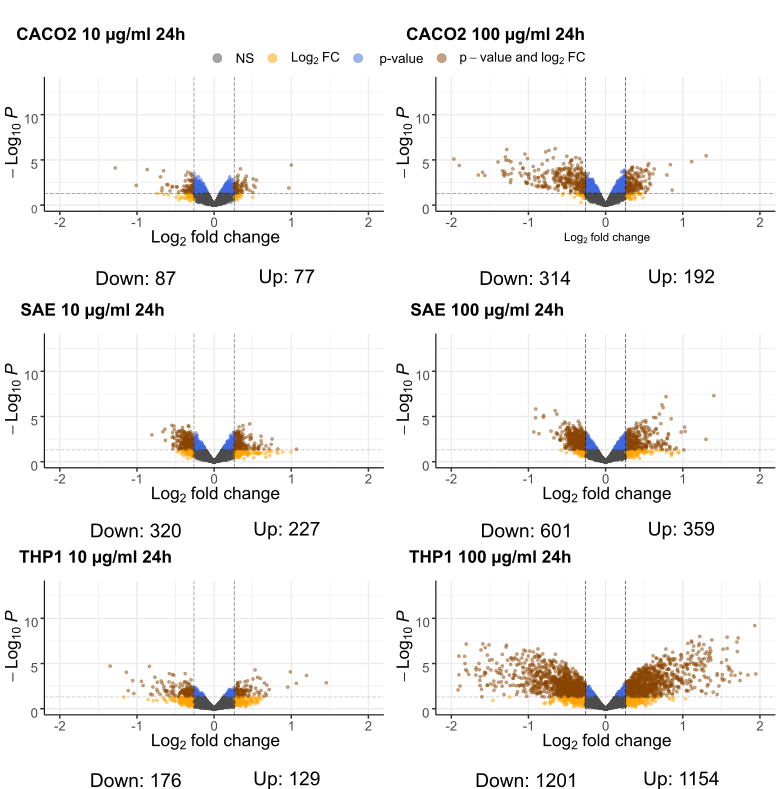
\includegraphics[width=0.83\linewidth]{fig1.png}
  \caption{\hl{Gene} %MDPI: please modify hyphen into minus in the image, same as in other figures.
% Reply: ???
 expression volcano plots for different {cellular models} and TiO\textsubscript{2}-nanobelt concentrations.
   On the x-axis log\textsubscript{2} (fold change) is depicted whereas on the y-axis the \hl{-}%MDPI: please confrim if this should be minus sigh $-$.
%Reply: Correct.
log\textsubscript{10} (\emph{p}-value) is depicted. The~dotted lines represent cut-off values for significantly changed genes (log\textsubscript{2} fold change $>$ 0.26 or $<$ $-$0.26, \emph{p}-value $<$ 0.05). A brown color depicts that a gene meets both cut-off criteria, a~blue color relates to meeting only the \emph{p}-value cut-off, an~orange color relates to meeting only the log$_{2}$ fold change cut-off, and a gray color indicates that a gene does not meet any of the criteria.}
\label{fig:fig1}
\end{figure}
\begin{paracol}{2}
%\linenumbers
\switchcolumn
\vspace{-12pt}

\subsection{Pathway Analysis}
Using the differentially expressed genes from the different {cellular models}, an overrepresentation analysis was performed to identify altered pathways after TiO\textsubscript{2}-nanobelt exposure. The~number of significantly overrepresented pathways (\emph{p}-value $<$ 0.05) is shown in Table~\ref{tab:tab1} in the column “Significant”. Concordant to the increase in differentially expressed genes matching our criteria shown in Figure~~\ref{fig:fig1}, the~number of resulting pathways increases with {an increase} in the concentration of TiO\textsubscript{2}-nanobelts. {While} there was a smaller increase in differentially expressed genes, we found a similar increase in resulting pathways for the SAE cell line. There was also an increase in the number of genes found for the {Caco-2/HT29-MTX co-culture; however,} it did not directly translate to an increase in overrepresented pathways. Although~overrepresentation analysis provides a great overview of all processes that are affected, it takes time to go manually over the many overrepresented pathways. Therefore, an~automated method to select desired pathways, i.e.,~toxicity-related pathways, provides a new approach to interpreting the~data. 

\begin{specialtable}[H]
\caption{Table listing the number of significantly overrepresented pathways, altered toxicity pathways, and the number of altered toxicity pathways for each~GO-term.}\label{tab:tab1}
\resizebox{\columnwidth}{!}{%
\begin{tabular}{lcccccc}
\toprule
 & \textbf{Significant} & \textbf{Toxicity} & \textbf{Apoptosis} & \textbf{Inflammation} & \textbf{\begin{tabular}[c]{@{}c@{}}DNA \\ Damage\end{tabular}} & \textbf{\begin{tabular}[c]{@{}c@{}}Oxidative \\ Stress\end{tabular}} \\ \midrule
\textbf{Pathways} & 1076 & 101 & 66 & 15 & 28 & 2 \\ \midrule
{Caco-2/HT29-MTX} low & 56 & 10 & 5 & 0 & 5 & 0 \\
{Caco-2/HT29-MTX} high & 58 & 10 & 10 & 1 & 0 & 0 \\ \midrule
SAE low & 28 & 3 & 1 & 0 & 2 & 0 \\
SAE high & 50 & 15 & 6 & 1 & 8 & 0 \\ \midrule
THP1 low & 38 & 10 & 9 & 4 & 0 & 0 \\
THP1 high & 201 & 39 & 31 & 9 & 3 & 1 \\\bottomrule
\end{tabular}%
}
\end{specialtable}
\vspace{-12pt}



\subsection{Toxicity-Related Pathways}
To gain more insight into the toxicity-related processes, the~overrepresented pathways were further categorized into pathways related to the apoptotic process, inflammatory response, DNA damage response, and/or oxidative stress. Often this kind of clustering of the pathways is performed manually. However, we implemented a gene-based approach. First, gene sets of four Gene~Ontology~(GO) terms were obtained, i.e.,~“apoptotic process”~(GO\hl{:}0006915, %MDPI: please confirm if space should be added after ``:''.
%Reply: Should not be added.
1269 genes), “inflammatory response”~(GO\hl{:}0006954, 569 genes),  “cellular response to DNA damage stimulus”~(GO\hl{:}0006974, 762 genes), and~“response to oxidative stress”~(GO\hl{:}0006979, 243 genes). Evidently, these processes are tightly connected. Whereas some can be causative for others, they are expected to overlap. Additional Figure~\ref{fig:figA1} shows the gene overlap between the four GO gene sets in a Venn diagram. Next, we calculated the gene overlap between the pathways from the WikiPathways pathway collection with the annotated genes of the four GO-terms. The~overlap was calculated by dividing the number of toxicity-related genes present in the pathway by the total number of genes present in the pathway. As~a cut-off we used 50$\%$ indicating that at least half of the pathway is directly linked to the GO-term of interest via their gene~overlap.

To select the desired gene overlap cut-off, we compared four cut-offs with each other and an overrepresentation analysis approach to see how many pathways these would give. The~cut-offs we used were 50\%, 60\%, 70\%, and 80\%. For~the overrepresentation analysis we looked for overrepresentation of the pathway genes in the gene lists of the GO-terms. The~results are shown in additional Table~\ref{tab:tabA1}. The~overrepresentation analysis \mbox{(\emph{p}-value~\hl{$<$}~0.05)} %Please confirm if this is correct.
%Reply: Was incorrect and it should be a single less than sign;
%       removed redundant <.
showed the most pathways to be linked to the four GO-terms; in~this case it showed 401, 250, 203, and 205 pathways overrepresented for the apoptotic process, inflammatory response, DNA damage, and oxidative stress GO-terms, respectively. The~80\% and 70\% gene overlap resulted in almost similar amounts of pathways compared to each other. They even resulted in 0 pathways for the inflammatory response GO-term. Moreover, it stands out that for the gene overlap approach only one pathway meets at least 50\% or higher gene overlap with the oxidative stress GO-term. Additionally, it is interesting to see that an overrepresentation analysis prompts hundreds of pathways compared to just dozens when looking at gene overlap. Comparing the results of the overrepresentation analysis and various cut-offs, the at least 50\% gene overlap cut-off was deemed best for our~approach. 

After this filtering step we found that, out of the 1076 pathways in the human pathway collection, 66 pathways are related to the apoptotic process, 15 are linked to inflammatory response, 28 are linked to DNA damage, and 2 are linked to oxidative stress.
It is noticeable that there are only two oxidative stress pathways, i.e.,~Detoxification of Reactive Oxygen Species~(wikipathways:WP2824~\cite{WP2824})
%MDPI: added space, please confirm.
%Reply: Must not be added. Have a look at: https://doi.org/10.1038/sdata.2018.29 for reference.
and Oxidative Stress~(wikipathways:WP408~\cite{WP408}), that have at least 50$\%$ of their genes overlapping with the genes annotated to the GO-term ``response to oxidative stress''. Based on this finding we can argue that most pathways in the pathway database we have used describe different processes that result in oxidative stress or where oxidative stress is part of/has an influence on the process itself. However, these do not describe oxidative stress as a process.  Nevertheless, these pathways are of interest for our~analysis. 

\subsection{Study Effect on Toxicity-Related Pathways}
The number of altered toxicity-related pathways is shown in Table~\ref{tab:tab1}. The~overrepresentation analysis was performed using the differentially expressed genes (log$_{2}$ fold change lower than $-$0.26 or greater than 0.26 and \emph{p}-value lower than 0.05). 

The {Caco-2/HT29-MTX co-culture} shows for both concentrations 10 overrepresented pathways. The SAE {cells} show 3 for the low concentration, which could be an indication of a very small toxic response to the TiO\textsubscript{2}-nanobelt exposure, and~15 for the high concentration. The~THP1 cell line shows a clear toxic response activation for the high concentration with 39 overrepresented pathways, and~10 for the low~concentration.



Importantly, while molecular pathways describe a process on a detailed level, their boundaries are often not clearly defined. Pathways are not independent, and~they interact with each other through shared genes or sub-pathways. Figure~\ref{fig:fig2} shows the gene overlap between the altered toxicity-related pathways in pathway-gene networks and highlights the differences in response between the cell lines. Pathways that cluster together indicate that these pathways depict similar biological processes with a high gene overlap. In~the following sections, the~biological pathways affected in the different cell lines will be discussed in~detail.




\subsection{{Caco-2/HT29-MTX} Cells}
While for both concentrations the {Caco-2/HT29-MTX co-culture} shows the same number of overrepresented pathways, the~pathways compared between the low and high concentrations are not all the same. Of~the ten pathways, three are found for both concentrations, namely IL-5 Signaling pathway (wikipathways:WP127,~\cite{WP127}), IL-2 Signaling pathway (wikipathways:WP49,~\cite{WP49}) and Endometrial Cancer (wikipathways:WP4155,~\cite{WP4155}). 
Interestingly, for the low concentration the pathways related to DNA-damage and repair show up in the results. %check meaning has been retained. Added two words to retain the meaning of the sentence.
For~example, HDR Through Homologous Recombination (HRR) or Single Strand Annealing (SSA) (wikipathways:WP3567,~\cite{WP3567}), Nonhomologous End-Joining (NHEJ) (wikipathways:WP3550,~\cite{WP3550}), and DNA Double-Strand Break Response (wikipathways:WP3543,~\cite{WP3543}) are among these pathways. However, for the high concentration it is interesting to see that the Apoptosis pathway (wikipathways:WP254,~\cite{WP254}) shows up, which could be an indication of {Caco-2/HT29-MTX} cells possibly undergoing apoptotic processes upon exposure to TiO\textsubscript{2}-nanobelts. However, these results indicate that the studied processes in {Caco-2/HT29-MTX co-cultures} are not extensively affected by the administration of TiO\textsubscript{2}-nanobelts, for~either the low or the high concentration. This finding supports the conclusion based on the cell viability assay results in the original study, which showed that there was no significant decrease in cell viability for the {Caco-2/HT29-MTX co-culture} for both concentrations of TiO\textsubscript{2}-nanobelts~\cite{Tilton2013}. 

\begin{figure}[H]
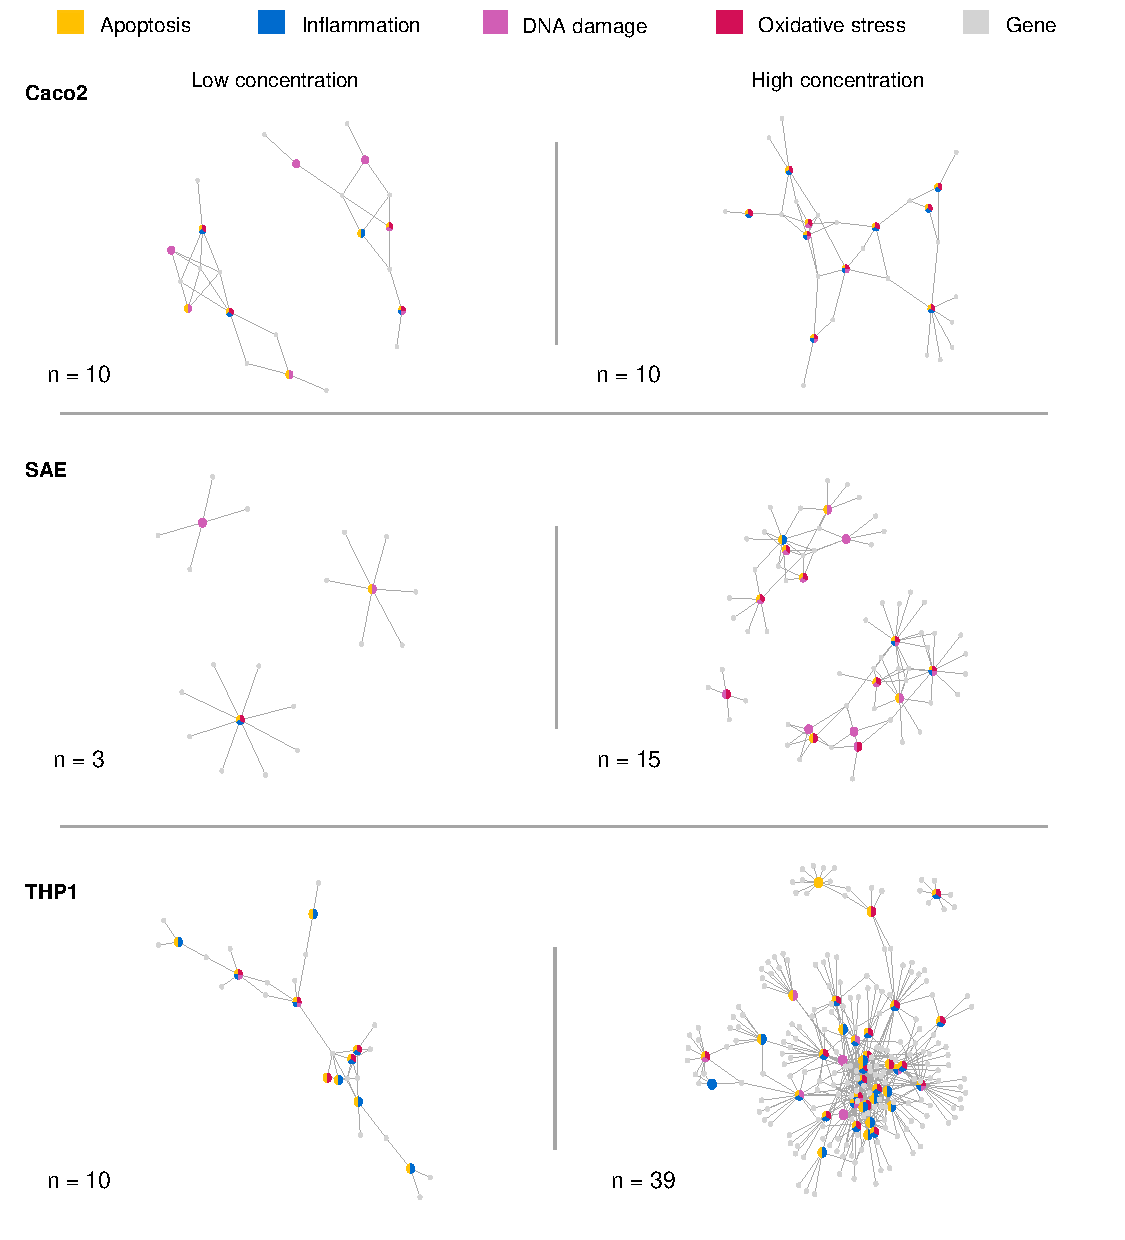
\includegraphics[width=1\linewidth]{fig2.pdf}
  \caption{Pathway-gene networks of altered toxicity-related pathways.
   The color of the nodes indicates to which GO-term the pathway is affiliated. Orange indicates apoptosis, blue indicates inflammation, pink indicates DNA-damage, and 
   red %check meaning has been retained. Correct.
   indicates oxidative stress. Gray nodes represent genes. Number (n) represents the number of significantly overrepresented pathways that are depicted in the networks.}
\label{fig:fig2}
\end{figure}
\unskip
\subsection{SAE Cells}
For the SAE cell line, the~low concentration only prompted three overrepresented pathways compared to 15 for the high concentration. Noticeable as well, only one of those three pathways was found to be overrepresented also for the high concentration, namely HDR through Homologous Recombination (HRR) or Single Strand Annealing (SSA) (wikipathways:WP3567,~\cite{WP3567}). This increase in pathways with a significantly increased overrepresentation of affected genes is an indication that upon exposure to the high concentration of TiO\textsubscript{2}-nanobelts, more biological processes related to toxicity are affected compared to the low~concentration. 

Next, for~the SAE cell line exposed with the low concentration, we found three overrepresented pathways. As~for the high concentration we found 15 overrepresented pathways. This increase in pathways with a significantly increased overrepresentation of affected genes is an indication that more biological processes related to toxicity are affected compared to the low concentration upon exposure to the high concentration of TiO\textsubscript{2}-nanobelts . For~the low concentration the pathways HDR through Homologous Recombination (HRR) or Single Strand Annealing (SSA) (wikipathways:WP3567,~\cite{WP3567}), IL-6 Signaling pathway (wikipathways:WP364,~\cite{WP364}), and Regulation of TP53 Activity through Phosphorylation (wikipathways:WP3838,~\cite{WP3838}) are overrepresented. The~first pathway describes a process of DNA double-strand break repair, where the second pathway describes the signaling of the cytokine IL-6 and the last pathway describes the regulation of TP53. Except~for the first pathway, which is also found in the result for the high concentration, the~overrepresented pathways describe more general regulatory pathways rather than detailed process-describing pathways. However, for~the high concentration we see multiple pathways related to DNA damage, such as the aforementioned HDR through Homologous Recombination (HRR) or Single Strand Annealing (SSA) (wikipathways:WP3567,~\cite{WP3567}), DNA IR-damage and Cellular Response via ATR (wikipathways:WP4016,~\cite{WP4016}), DNA IR-Double Strand Breaks (DSBs) and Cellular Response via ATM (wikipathways:WP3959,~\cite{WP3959}), and DNA Mismatch Repair (wikipathways:WP531,~\cite{WP531}) among others. Moreover, the results prompted apoptosis-related pathways such as Apoptosis Modulation and Signaling (wikipathways:WP1772,~\cite{WP1772}) and Apoptosis Modulation by HSP70 (wikipathways:WP384,~\cite{WP384}). This is also an indication that the high concentration induced more distinct biological processes related to toxicity compared to the low concentration for the SAE cell~line. 

\subsection{THP1 Cells}
For the THP1 cell line, there are only 10 significantly overrepresented pathways for the low concentration of TiO\textsubscript{2}-nanobelts. However, among~these pathways, the~pathways TNF Signaling (wikipathways:WP3380,~\cite{WP3380}), Apoptosis (wikipathways:WP254,~\cite{WP254}), Apoptotic Execution Phase (wikipathways:WP1784,~\cite{WP1784}), TNF alpha Signaling Pathway (wikipathways:WP231,~\cite{WP231}), and TNF-related Weak Inducer of Apoptosis (TWEAK) Signaling pathway (wikipathways:WP2036,~\cite{WP2036}) are present. This indicates that upon exposure to the low concentration of TiO\textsubscript{2}-nanobelts the THP1 cell line activates immune- and inflammation-related processes. This result can be explained as a general cell activity response since THP1 is a macrophage-like cell line. However, it can also be explained due to the effect of TiO\textsubscript{2}-nanobelts on the THP1 cell line in this case. TiO\textsubscript{2}-nanobelts are likely to induce toxic processes, even at a low concentration, which results in an inflammatory response of the THP1 cells. Similar inflammatory responses, like activation of Nf-$\kappa$B and production of TNF-$\alpha$, were seen in these cells upon exposure to other nanoparticles such as ZnO NM-110, SiO\textsubscript{2} NM-200, and Ag NM-300~\cite{Brzicova2019}. 

Compared to the low concentration, the~high concentration yields more pathways with significant overrepresentation i.e.,~39 versus 10. Except~for the pathway Apoptotic Execution Phase (wikipathways:WP1784,~\cite{WP1784}) all other 9 pathways which showed up for the low concentration were found for the high concentration as well. In~addition to these pathways, pathways such as Oxidative Stress (wikipathways:WP408,~\cite{WP408}), Nanoparticle Triggered Regulated Necrosis (wikipathways:WP2513,~\cite{WP2513}), and Mismatch Repair (wikipathways:WP3381,~\cite{WP3381}) %please be consistent with capitalization of pathways throughout the paper (at present some have initial capitals and some do not). Changed to be consistent throughout manuscript.
and more were among the significant pathways. These results indicate that the THP1 cell line upon exposure to the high concentration of TiO\textsubscript{2}-nanobelts results in toxicity-related processes such as inflammation, DNA damage, and~oxidative stress. The~higher number of pathways that show up in the result together with the biological processes they depict indicate that the high concentration induces greater effects than the low concentration. This was also seen in the original paper where the low concentration induced a significant decrease in cell viability, while the high concentration induced an even greater decrease~\cite{Tilton2013}. Furthermore, it has also been shown that nanoparticles can activate similar processes, such as inflammatory processes and DNA damage, as~seen upon exposure to the high concentration~\cite{Brzicova2019,Huang2017}.

{The THP1 cell line is the cellular model that has the most inflammation-related pathways in the results: four for the low concentration and nine for the high concentration. All four of the low concentrations show up in the results of the high concentration as well. These pathways are Photodynamic-therapy-induced NF-kB Survival Signaling} (wikipathways:WP3617,~\cite{WP3617}), {Interleukin-10 Signaling} (wikipathways:WP4063,~\cite{WP4063}), {Fibrin Complement Receptor 3 Signaling Pathway} (wikipathways:WP4136,~\cite{WP4136}), {and Platelet-mediated Interactions With Vascular and Circulating Cells} (wikipathways:WP4462,~\cite{WP4462}).
{Nanoparticle-induced genotoxicity can arise and a distinction between primary and secondary genotoxicity can be made. Inflammation drives secondary toxicity as suggested by} Emma Åkerlund~et~al., {who showed that conditioned media from differentiated THP1 cells induced DNA-damage in HBEC after} 3~h~exposure~\cite{Akerlund2019}. {While there are inflammatory-related pathways in the results for the THP1 cell line, only the high concentration has three DNA-damage-related pathways in the results. The~presence of DNA-damage-related pathways and inflammatory-related pathways could indicate secondary genotoxicity for the THP1 cells upon exposure to the high concentration. However, more research is needed to address this exact mechanism.} 

\subsection{Comparison Between Cell Lines}
The focused analysis of alterations in toxicity-related processes showed differences between the three cell lines and the concentrations studied. It has been reported before that the molecular response depends on the cell type and concentration~\cite{TadaOikawa2016}. 

{Caco-2/HT29-MTX} cells seem resilient to the exposure and show very little activation of toxicity-related processes. {While for this dataset a co-culture was used,} the passage of nanoparticles through the cellular barriers of {Caco-2} cells has been shown to be limited, which could result in reduced uptake and therefore less toxic response~\cite{Ye2017}. {This could partially explain the resilience we see in our results.} Subsequently, this indicates a lower importance of gastro-intestinal uptake in general {but no direct conclusions could be made based on the results and information we have.} However, TiO\textsubscript{2}-nanobelts caused the biggest toxicological response to THP1 cells, as they are more sensitive to exposure compared to epithelial cell lines RLE-6TN and BEAS-2B~\cite{Xia2013}. Moreover, it has been reported that this response is specific to the nanobelt form of TiO\textsubscript{2}~\cite{Xia2013}.

Interestingly, approximately 10\% of the pathways in WikiPathways and Reactome can be categorized as toxicity-related, in~other words these pathways have at least 50\% gene overlap with the GO terms we selected. This highlights the fundamental cellular processes involved but could also indicate a bias in the pathway collections towards these well-studied processes. Nonetheless, these pathways are considered important pathways, hence they are studied~well.  

To illustrate how the effects can be studied in more depth we visualized the log fold change of all six conditions on the Oxidative Stress pathway (wikipathways:WP408~\cite{WP408}), the~Apoptosis pathway (wikipathways:WP254~\cite{WP254}), and the DNA Mismatch Repair pathway (wikipathways:WP531~\cite{WP531}). This shows that for most genes in these pathways gene expression data are present (see additional Figures~\ref{fig:figA2} and~\ref{fig:figA3}). 

While the Oxidative Stress pathway shown in Figure~\ref{fig:fig3} only shows up to be significantly overrepresented for the THP1 cell line for the high concentration, it is still an interesting pathway to dive deeper into. The~NFKB1 gene, which encodes for the Nf$\kappa$B-p105 subunit, has the highest log fold change for the THP1 cell line, high concentration. Additionally, the~THP1 cell line, low concentration, shows a positive log fold change as well, whereas the SAE cell line shows negative log fold changes and the {Caco-2/HT29-MTX co-culture} shows noticeably lower positive log fold changes for both concentrations. Furthermore, the~SOD2 gene, which is involved in the conversion of superoxide and protects against oxidative stress, shows a similar pattern~\cite{Urso2003}. These genes indicate that the THP1 cell line responds to oxidative stress by increasing the expression of protective~genes. 


Moreover, the~Apoptosis pathway shows positive log fold changes of the CASP2 and CASP7 genes, which are involved in apoptosis execution, for~the SAE and THP1 cell lines for both concentrations whereas the {Caco-2/HT29-MTX co-culture} shows no negative or positive log fold change~\cite{BouchierHayes2011,Lamkanfi2010}. Furthermore, the~pathway shows positive log fold changes for the apoptosis-promoting interferon regulatory factors such as IRF4 and IRF5~\cite{Stang2007,Fanzo2003,Hu2009}, which is a similar pattern as described for the CASP2 and CASP7 genes. This could be an indication that apoptosis is stimulated in these cell lines. However, the~original study by Tilton~et~al. does not show a significant decrease in cell viability. 
The DNA Mismatch Repair pathway shows a positive log fold change {for the LIG1 gene}, which encodes for DNA ligase 1 {for both the Caco-2/HT29-MTX and THP1 cells}. This enzyme is involved in both DNA replication and in this context more importantly repair~\cite{Mota2019}. The~aforementioned genes show positive log fold changes for the THP1 cell line throughout the pathway. The~increase in expression of these genes could be an indication that DNA mismatch repair is activated due to exposure to TiO\textsubscript{2}-nanobelts.

\begin{figure}[H]
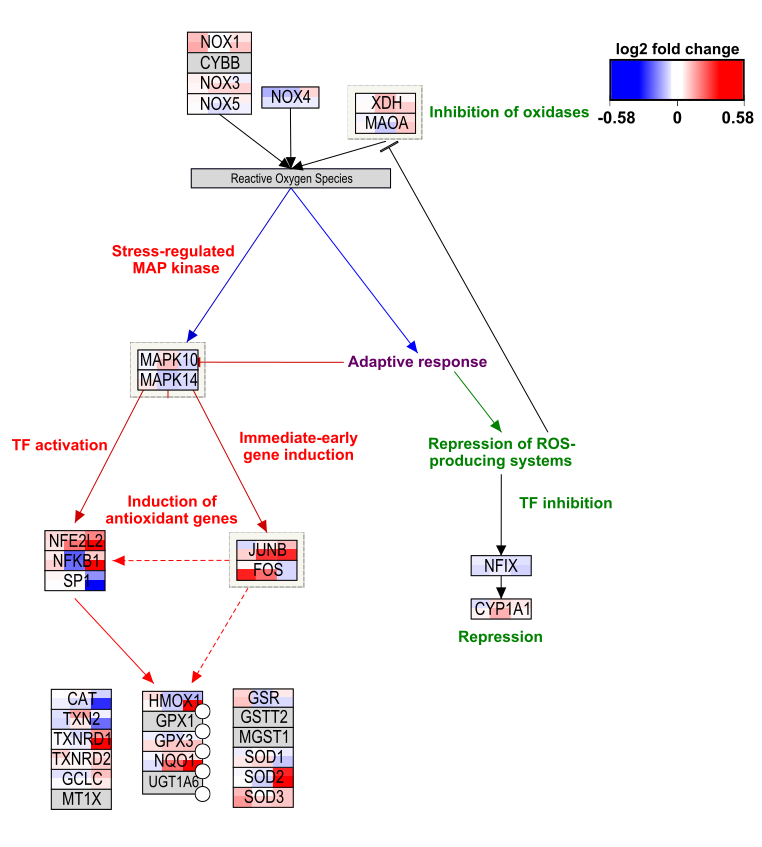
\includegraphics[height=14cm,keepaspectratio]{fig3.png}
  \caption{\hl{Visualization} of log fold change on the Oxidative Stress pathway (wikipathways:WP408) for all six conditions.
{Cellular models} are depicted from left to right as {Caco-2/HT29-MTX}, SAE, and THP1. The~top row depicts the low concentrations whereas the bottom row depicts the high concentrations. {Color gradient for differential gene expression after exposure goes from blue (downregulated) via white (not changed) to red (upregulated).}}
\label{fig:fig3}
\end{figure}
\vspace{-12pt}

\subsection{The Advantage of Our Approach}
Enrichment analysis for gene expression data is well-established and can easily be automated to increase reproducibility~\cite{Yu2012}. The~interpretation of the long list of altered, often overlapping, pathways is still a challenge. {To mitigate this challenge we proposed} an automated approach to filter the pathway enrichment result towards a specific biological focus, in~this case toxicity. A~more context-specific interpretation is facilitated {using GO-term gene sets of interest}. The~generated pathway-gene networks showcase the connectedness of the processes and provide a more systemic view than looking at individual pathways. The~approach yields a fast and easy method with which to select pathways of interest for more detailed scrutiny, as~we have shown. While interpretation and comparison between multiple datasets on a process level are still challenging, the~automated analysis workflow used supports the exploration of the data~\cite{TiO2-scripts}. {Our approach showed the biological response of the three cellular models on a biological process level, making use of pathways. Using pathways to investigate the response not only highlights biological processes that are affected, but~also enables researchers to dive deeper into the pathways on a gene-level. We showed this in our research, where we could easily discuss affected genes in relation to biological processes based on the results we retrieved from our approach. Furthermore, our approach is suitable for quickly retrieving results towards specific biological processes, which will aid researchers in their future research. Moreover, our approach is suitable for quick reanalysis each time new pathway knowledge is discovered, thus pathway databases are~updated.}

%%%%%%%%%%%%%%%%%%%%%%%%%%%%%%%%%%%%%%%%%%
\section{Conclusions}
In this study we investigated the molecular response of three different cell lines to exposure to TiO\textsubscript{2}-nanobelts. Using our process-level analysis based on pathway analysis {in combination with the use of} gene sets and~network visualization, our findings support the results by S.C. Tilton~et~al. showing that the three {cellular models, Caco-2/HT29-MTX}, SAE, and~THP1, show different toxicity-related responses to the exposure of TiO\textsubscript{2}-nanobelts from resilient {Caco-2/HT29-MTX} and SAE cells to strongly responding THP1 cells. The~latter is not unexpected since the observed effects align with the biological function of these immune cells. Importantly, the~approach allowed us not {only} to find changes in gene expression, but~also to find responding molecular pathways via the pathway analysis. Additionally, {it} allowed us to filter the broad pathway enrichment results to a focused view on the cytotoxic processes affected. {The filtering steps we included in our workflow allow a very targeted approach.} This allows us to visualize and explore the interactions between responding genes, based on underlying molecular processes {in greater detail and in a less time-consuming manner.  The~approach is suitable for quick reanalysis of datasets each time pathway databases are updated with newly discovered pathway knowledge. Moreover,} this versatile approach captured in the R-script can easily be adapted to isolate other processes by using other Gene Ontology terms diverting the focus to other biological processes of~interest.
%%%%%%%%%%%%%%%%%%%%%%%%%%%%%%%%%%%%%%%%%%
\section{Materials and~Methods}
\unskip

\subsection{Dataset}
In this study, a~published and publicly available transcriptomics dataset generated by Tilton~{et al.}~\cite{Tilton2013} was used. The~dataset is available from the Gene Expression Omnibus (accession number: GSE42069)~\cite{Edgar2002}. Quality control, data pre-processing, and~statistical analysis were performed using scripts from ArrayAnalysis.org~\cite{Eijssen2013}. 

The dataset consisted of 18 samples from three human-like {cellular models}, i.e.,~{Caco-2/HT29-MTX}, SAE, and~THP1, which were exposed to either medium (control), 10~$\upmu$g/mL or 100~$\upmu$g/mL TiO\textsubscript{2}-nanobelts for 24 h in triplicate. {To run the same analysis for the 1 h time point the workflow in the 1h repository can be} used~\cite{TiO2-scripts-1h}. {The number of samples, cellular models, and number of replicates were the same for the 1 h time point compared to the 24 h time point.} Culture conditions were kept as identical as possible between the three cell lines {for both time points}. Details can be found via the original publication by \mbox{Tilton~{et al.}~\cite{Tilton2013}.}

Volcano plots depicting differential gene expression were made using the EnhancedVolcano package (version 1.4.0) for R (version 3.6.1)~\cite{R2020,VolcanoPlot}. Genes were considered differentially expressed between treated and control when they had an absolute fold change greater than 1.2 (log$_{2}$ fold change lower than $-$0.26 or higher than 0.26) and a \emph{p}-value lower than~0.05. 

\subsection{Pathway Analysis}
Overrepresentation analysis was performed using the enricher function of the clusterProfiler package (version 3.14.3)~\cite{Yu2012} for R to identify the molecular changes on a pathway level. The~human pathway collection containing 1076 pathways was obtained from WikiPathways (\url{http://www.wikipathways.org} \hl{(accessed on 2021-08-28),} %MDPI: please add access date.
%Reply: date in ISO standard format
%MPDI: please check out: https://chem-bla-ics.blogspot.com/2021/08/scholarly-journals-should-use-archived.html (consider this a feature request)
 version 20201003,~\cite{Martens2020}). The~Curated and Reactome collections from WikiPathways were included in the analysis. Enrichment analysis was performed for differentially expressed genes using the fold change and \emph{p}-value cutoff as described in the previous section. Additionally, default settings of the enricher function of the clusterProfiler package were used, except \emph{p}-value and q-value (false discovery rate) cutoff were set to 1 to include all results at this stage. This allowed us to later select the desired results based on a \emph{p}-value smaller than 0.05. Minimal gene set size was set to 10 and the maximum gene set size was set to~300.

\subsection{Toxicity-Related Processes}
Within the two human pathway collections used, toxicity-related pathways were identified based on the gene overlap with the toxicity-related gene sets. The~overlap was calculated by dividing the number of toxicity-related genes present in the pathway by total number of genes present in the pathway. The~gene sets were retrieved from the Gene Ontology (GO, version: release 2020-06) for the following four toxicity-related GO-terms: “apoptotic process” (GO:0006915), “inflammatory response” (GO:0006954), “cellular response to DNA damage stimulus” (GO:0006974), and “response to oxidative stress” (GO:0006979)~\cite{Ashburner2000,Carbon2020}. Associated genes were retrieved using the biomaRt package in R (version 2.42.0, Ensembl Genes 100)~\cite{Durinck2005,Durinck2009}. Using the GO evidence codes, only genes with experimental evidence or manually curated annotations were included to ensure high confidence that the gene was involved in the specific process (IBA, IC, IDA, IEP, IGI, IMP, IPI, TAS, \url{http://geneontology.org/docs/guide-go-evidence-codes/} \hl{(accessed on 2021-08-28),}
%Reply: date added
see additional Table~\ref{tab:tabA2}). Gene overlap between GO terms was visualized using Venny version 2.1.0~\cite{Venny}. 

\subsection{Network Visualization}
Altered pathways in the enrichment analysis were filtered for toxicity-related pathways and then visualized as pathway-gene networks to portray the overlap and crosstalk between the pathways. To~construct the networks, edge (source: pathway, target: gene) and node (all unique source and target nodes) files were created of the altered pathways. The~networks were made using the igraph R package (version 1.2.4.1)~\cite{Csardi2006}.

\subsection{Reproducible Analysis Workflow}
The complete analysis is automated in R (version 3.6.3) and can easily be repeated with a new transcriptomics dataset or different selection focus. The~R scripts are available on GitHub (\url{https://github.com/laurent2207/TiO2-scripts} \hl{(accessed on 2021-08-28)}) and archived on Zenodo~\cite{TiO2-scripts}.
%Reply: date added

%%%%%%%%%%%%%%%%%%%%%%%%%%%%%%%%%%%%%%%%%%

%\section{Patents}

%This section is not mandatory, but may be added if there are patents resulting from the work reported in this manuscript.

%%%%%%%%%%%%%%%%%%%%%%%%%%%%%%%%%%%%%%%%%%
\vspace{6pt} 

%%%%%%%%%%%%%%%%%%%%%%%%%%%%%%%%%%%%%%%%%%
%% optional
%\supplementary{The following are available online at \linksupplementary{s1}, Figure S1: title, Table S1: title, Video S1: title.}

% Only for the journal Methods and Protocols:
% If you wish to submit a video article, please do so with any other supplementary material.
% \supplementary{The following are available at \linksupplementary{s1}, Figure S1: title, Table S1: title, Video S1: title. A supporting video article is available at doi: link.} 

%%%%%%%%%%%%%%%%%%%%%%%%%%%%%%%%%%%%%%%%%%
\authorcontributions{Conceptualization, L.A.W., E.L.W., C.T.E., and M.K.; methodology, L.A.W., E.L.W., C.T.E., and M.K.; software, L.A.W. and M.K.; validation, L.A.W. and M.K.; formal analysis L.A.W. and M.K.;  investigation, L.A.W.; resources, L.A.W., E.L.W., and M.K.; data curation, L.A.W. and M.K.; writing---original draft preparation, L.A.W., E.L.W., C.T.E., and M.K.; writing---review and editing, L.A.W., E.L.W., C.T.E., and~M.K.; visualization, L.A.W. and M.K.; supervision, E.L.W. and C.T.E.; project administration, L.A.W.; funding acquisition, E.L.W. All authors have read and agreed to the published version of the~manuscript.}

\funding{\textls[-15]{This work received funding from the European Union’s Horizon 2020 research and innovation programme via the NanoCommons Project under grant agreement No. 731032 (L.A.W. and E.L.W.)}}

\institutionalreview{Not applicable.}

\informedconsent{Not applicable.}

\dataavailability{Data analyzed in this paper are from the publicly available dataset generated by Tilton~{et al.}~\cite{Tilton2013} (accession number: GSE42069)~\cite{Edgar2002}.} 

\acknowledgments{We would like to thank Susan C Tilton, Norman J Karin, Ana Tolic, Yumei Xie, Xianyin Lai, Raymond F Hamilton Jr, Katrina M Waters, Andrij Holian, Frank A Witzmann, and~Galya Orr for the original article that generated the data used in this paper (\url{https://doi.org/10.3109/17435390.2013.803624} \hl{(accessed on 2021-08-28)}).
%Reply: date added
Furthermore, we would like to thank Marvin Martens (\url{https://orcid.org/0000-0003-2230-0840} \hl{(accessed on 2021-08-28)}) for the insightful discussion and his input.}
%Reply: date added

\conflictsofinterest{The authors declare no conflicts of~interest.} 

%% Optional
%\sampleavailability{Samples of the compounds ... are available from the authors.}

%%%%%%%%%%%%%%%%%%%%%%%%%%%%%%%%%%%%%%%%%%
%% Only for journal Encyclopedia
%\entrylink{The Link to this entry published on the encyclopedia platform.}

%%%%%%%%%%%%%%%%%%%%%%%%%%%%%%%%%%%%%%%%%%
%% Optional
\abbreviations{Abbreviations}{The following abbreviations are used in this manuscript:\\

\noindent 
\begin{tabular}{@{}ll}
TiO\textsubscript{2} & Titanium dioxide\\
SAE & Small airway epithelial cells\\
THP1 & Human monocytic cells\\
{Caco-2} & Human epithelial colorectal adenocarcinoma cells\\
GO & Gene Ontology\\
\end{tabular}}

%%%%%%%%%%%%%%%%%%%%%%%%%%%%%%%%%%%%%%%%%%
%% Optional
%\newpage
\appendixtitles{no} % Leave argument "no" if all appendix headings stay EMPTY (then no dot is printed after "Appendix A"). If the appendix sections contain a heading then change the argument to "yes".
\appendixstart
\appendix
\section{}

\setcounter{table}{0}
\renewcommand{\thetable}{A\arabic{table}}
\vspace{-6pt}



% Please add the following required packages to your document preamble:
% \usepackage{multirow}
\begin{specialtable}[H]
\caption{Table containing the number of pathways related to the four GO-terms. Based on either an overrepresentation analysis (\emph{p}-value $<$ 0.05), 80\% gene overlap, 70\% gene overlap, 60\% gene overlap, or 50\% gene overlap.
}
\label{tab:tabA1}
\resizebox{\columnwidth}{!} \\ \textbf{Gene Overlap}\end{tabular} & \begin{tabular}[c]{@{}c@{}}\textbf{70\%} \\ \textbf{Gene Overlap}\end{tabular} & \begin{tabular}[c]{@{}c@{}}\textbf{60\%} \\ \textbf{Gene Overlap}\end{tabular} & \begin{tabular}[c]{@{}c@{}}\textbf{50\%} \\ \textbf{Gene Overlap}\end{tabular} \\ \midrule
\begin{tabular}[c]{@{}l@{}}apoptotic process \\ (GO:0006915)\end{tabular} & 401 & 11 & 15 & 31 & 66 \\ \midrule
\begin{tabular}[c]{@{}l@{}}inflammatory response \\ (GO:0006954)\end{tabular} & 250 & 0 & 0 & 6 & 15 \\ \midrule
\begin{tabular}[c]{@{}l@{}}DNA damage \\ (GO:0006974)\end{tabular} & 203 & 15 & 20 & 23 & 28 \\ \midrule
\begin{tabular}[c]{@{}l@{}}oxidative stress \\ (GO:0006979)\end{tabular} & 205 & 1 & 1 & 1 & 1 \\ \bottomrule
\end{tabular}%
}
\end{specialtable}
\vspace{-12pt}


% Please add the following required packages to your document preamble:
% \usepackage[table,xcdraw]{xcolor}
% If you use beamer only pass "xcolor=table" option, i.e.,~\documentclass[xcolor=table]{beamer}
\begin{specialtable}[H]
\caption{\hl{List} %MDPI: Please confirm if the background color is necessary.
 of Gene Ontology (GO) evidence annotation codes that were used to remove genes related to the four GO terms with these annotations (bottom part). Additionally, the~annotation codes that were present are shown (top part).}
\label{tab:tabA2}
\renewcommand\arraystretch{1.18}
\resizebox{\columnwidth}{!}{%
\begin{tabular}{lll}
\toprule
\multicolumn{1}{c}{{\color[HTML]{000000} \textbf{Abbreviation}}} & \multicolumn{1}{c}{{\color[HTML]{000000} \textbf{Full Name}}} & \multicolumn{1}{c}{{\color[HTML]{000000} \textbf{Category}}} \\\hline
\rowcolor[HTML]{C0C0C0} 
IBA                                                              & Inferred from Biological aspect of Ancestor                   & Phylogenetically-inferred annotations                        \\
IC                                                               & Inferred by Curator                                           & Curator statement evidence codes                             \\
\rowcolor[HTML]{C0C0C0} 
IDA                                                              & Inferred from Direct Assay                                    & Experimental evidence codes                                  \\
IEP                                                              & Inferred from Expression Pattern                              & Experimental evidence codes                                  \\
\rowcolor[HTML]{C0C0C0} 
IGI                                                              & Inferred from Genetic Interaction                             & Experimental evidence codes                                  \\
IMP                                                              & Inferred from Mutant Phenotype                                & Experimental evidence codes                                  \\
\rowcolor[HTML]{C0C0C0} 
IPI                                                              & Inferred from Physical Interaction                            & Experimental evidence codes                                  \\
TAS                                                              & Traceable Author Statement                                    & Author statement evidence codes                              \\\hline
\multicolumn{3}{c}{\textbf{Removed annotations}}                                                                                                                                                \\\hline
\rowcolor[HTML]{C0C0C0} 
ND                                                               & No Biological Data Available                                  & Curator statement evidence codes                             \\
NAS                                                              & Non-traceable Author Statement                                & Author statement evidence codes                              \\
\rowcolor[HTML]{C0C0C0} 
IEA                                                              & Inferred from Electronic Annotation                           & Electronic annotation evidence code                          \\
ISS                                                              & Inferred from Sequence or structural Similarity               & Computational analysis evidence codes                        \\
\rowcolor[HTML]{C0C0C0} 
ISO                                                              & Inferred from Sequence Orthology                              & Computational analysis evidence codes                        \\
ISA                                                              & Inferred from Sequence Alignment                              & Computational analysis evidence codes                        \\
\rowcolor[HTML]{C0C0C0} 
ISM                                                              & Inferred from Sequence Model                                  & Computational analysis evidence codes                        \\
IGC                                                              & Inferred from Genomic Context                                 & Computational analysis evidence codes                        \\
\rowcolor[HTML]{C0C0C0} 
RCA                                                              & Inferred from Reviewed Computational Analysis & Computational analysis evidence codes\\ \noalign{\hrule height 1.0pt}
\end{tabular}%
}
\end{specialtable}
\unskip

\begin{figure}[H]
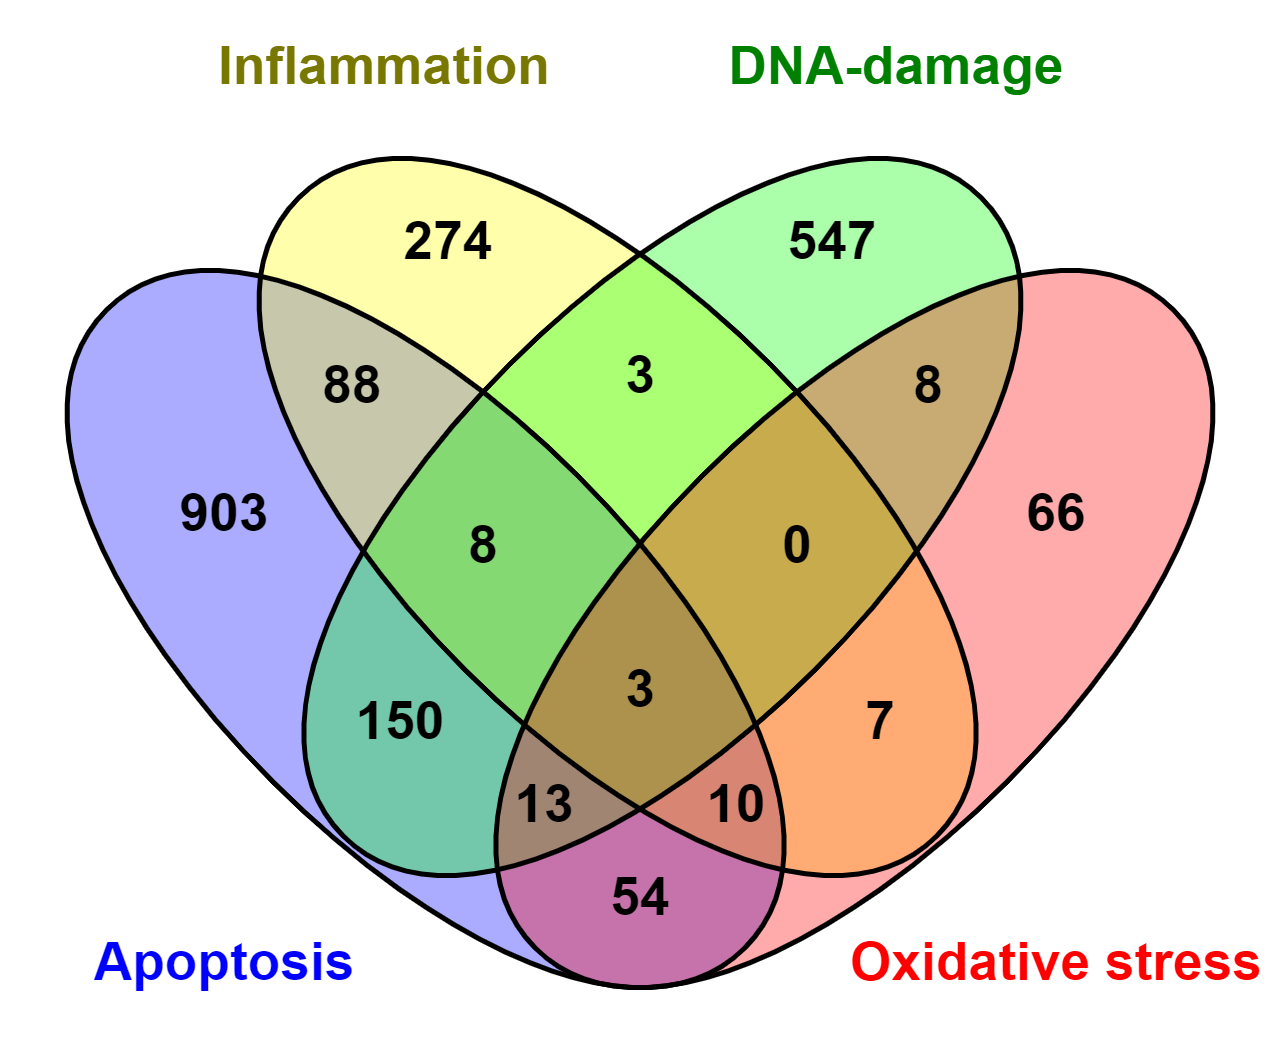
\includegraphics[height=8cm,keepaspectratio]{figA1.png}
\caption{Venn diagram showing the number of overlapping genes between the four GO-terms “apoptotic process”, “inflammation”, “cellular response to DNA damage stimulus”, “DNA damage and Oxidative~stress”.
}
\label{fig:figA1}
\end{figure}
\vspace{-12pt}

% start a new page without indent 4.6cm
\clearpage
%MDPI: please check if needed in final PDF
\end{paracol}
\nointerlineskip
\renewcommand{\thefigure}{A\arabic{figure}}
\begin{figure}[H]
\widefigure
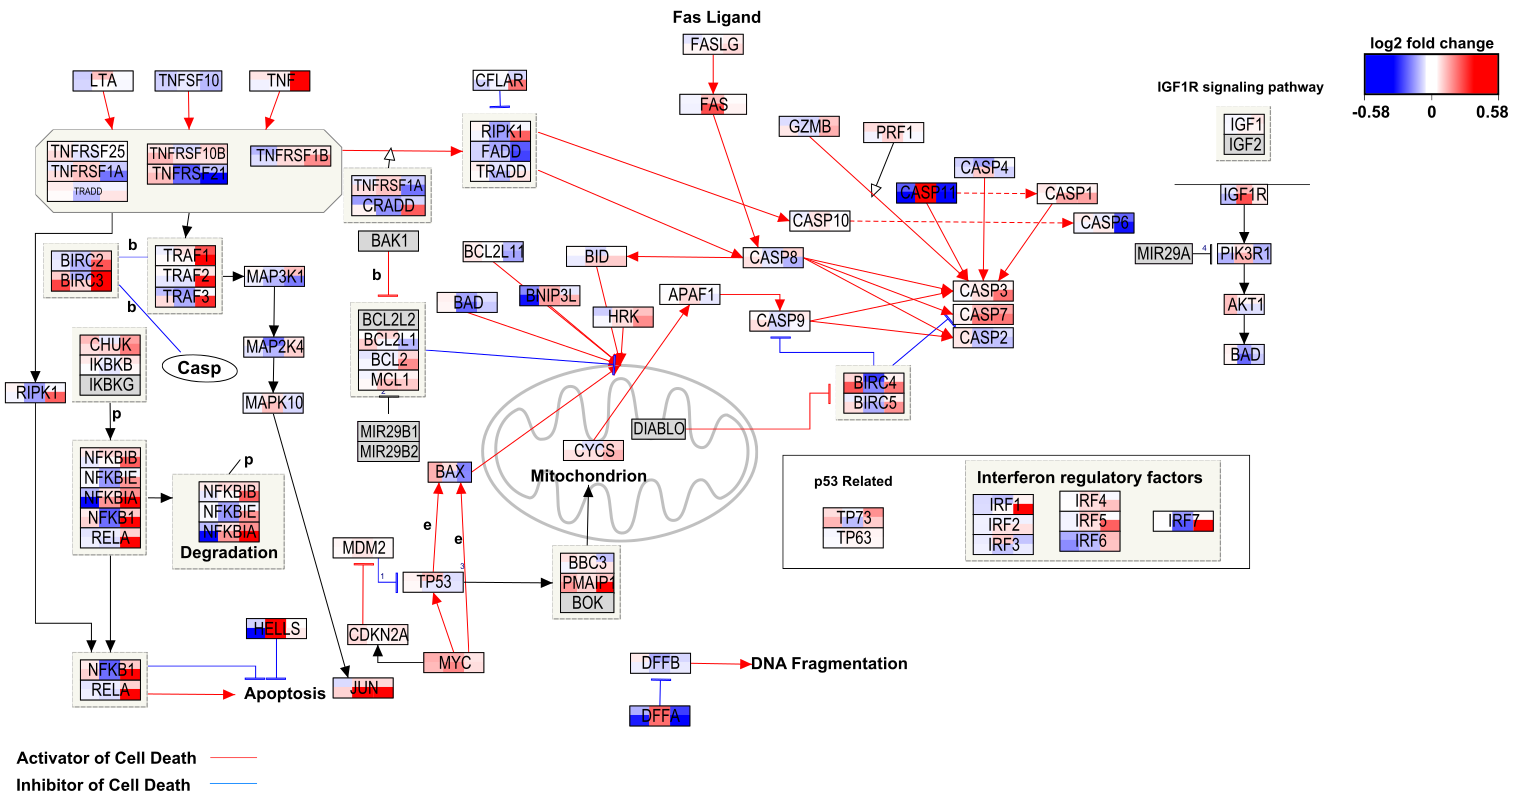
\includegraphics[height=9.5cm,keepaspectratio]{figA2.png}
\caption{\hl{Visualization} of log$_{2}$ fold change on the Apoptosis pathway (wikipathways:WP254) for all six conditions.
{Cellular models} are depicted from left to right as {Caco-2/HT29-MTX}, SAE, and THP1. The~top row depicts the low concentrations whereas the bottom row depicts the high concentrations. {Color gradient for differential gene expression after exposure goes from blue (downregulated) via white (not changed) to red (upregulated).}
}
\label{fig:figA2}
\end{figure}
\begin{paracol}{2}
%\linenumbers
\switchcolumn

\vspace{-12pt}

% start a new page without indent 4.6cm
\clearpage
\end{paracol}
\nointerlineskip
\begin{figure}[H]
\widefigure
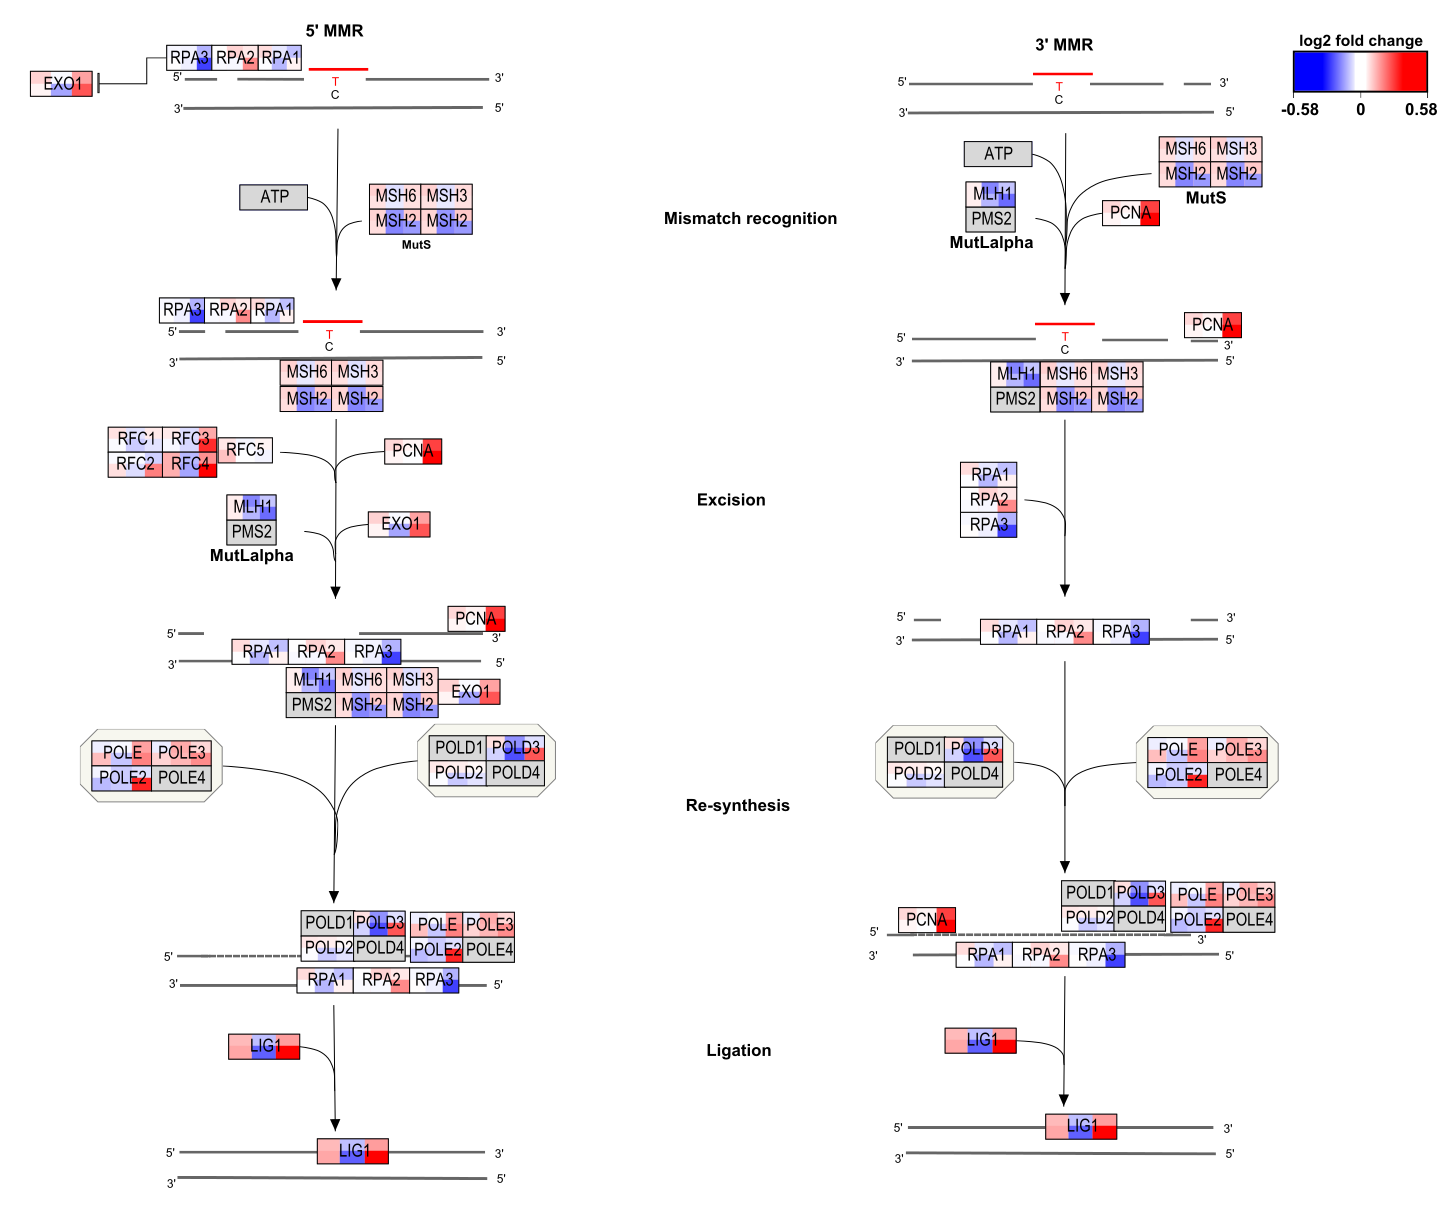
\includegraphics[height=15cm]{figA3.png}
\caption{\hl{Visualization} of log fold change on the DNA Mismatch Repair pathway (wikipathways:WP531) for all six conditions.
{Cellular models} are depicted from left to right as {Caco-2/HT29-MTX}, SAE, and THP1. The~top row depicts the low concentrations whereas the bottom row depicts the high concentrations. {Color gradient for differential gene expression after exposure goes from blue (downregulated) via white (not changed) to red (upregulated).}
}
\label{fig:figA3}
\end{figure}
\begin{paracol}{2}
%\linenumbers
\switchcolumn

%The appendix is an optional section that can contain details and data supplemental to the main text---for example, explanations of experimental details that would disrupt the flow of the main text but nonetheless remain crucial to understanding and reproducing the research shown; figures of replicates for experiments of which representative data are shown in the main text can be added here if brief, or as Supplementary Data. Mathematical proofs of results not central to the paper can be added as an appendix.

%\section{}
%All appendix sections must be cited in the main text. In the appendices, Figures, Tables, etc. should be labeled, starting with ``A''---e.g., Figure A1, Figure A2, etc. 

%%%%%%%%%%%%%%%%%%%%%%%%%%%%%%%%%%%%%%%%%%
\end{paracol}
%%%%%%%%%%%%%%%%%%%%%%%%%%%%%%%%%%%%%%%%%%
\reftitle{References}

% Please provide either the correct journal abbreviation (e.g. according to the “List of Title Word Abbreviations” http://www.issn.org/services/online-services/access-to-the-ltwa/) or the full name of the journal.
% Citations and References in Supplementary files are permitted provided that they also appear in the reference list here. 

%=====================================
% References, variant A: external bibliography
%=====================================
%\externalbibliography{yes}
%\bibliography{references}

%%%%%%%%%%%%%%%%%%%%%%%%%%%%%%%%%%%%%%%%%%
\begin{thebibliography}{999}

\bibitem[Ray \em{et~al.}(2009)Ray, Yu, and Fu]{Ray2009}
Ray, P.C.; Yu, H.; Fu, P.P.
\newblock Toxicity and Environmental Risks of Nanomaterials: Challenges and
  Future Needs.
\newblock {\em J. Environ. Sci. Health Part C} {\bf 2009},
  {\em 27},~1--35,
\newblock
  doi:{\changeurlcolor{black}\href{https://doi.org/10.1080/10590500802708267}{\detokenize{10.1080/10590500802708267}}}.

\bibitem[Shin \em{et~al.}(2015)Shin, Song, and Um]{Shin2015}
Shin, S.; Song, I.; Um, S.
\newblock Role of Physicochemical Properties in Nanoparticle Toxicity.
\newblock {\em Nanomaterials} {\bf 2015}, {\em 5},~1351--1365,
\newblock
  doi:{\changeurlcolor{black}\href{https://doi.org/10.3390/nano5031351}{\detokenize{10.3390/nano5031351}}}.

\bibitem[Vison{\`{a}} \em{et~al.}(2018)Vison{\`{a}}, Villani, Manzoni, Chen,
  Ardissino, Russo, Moretti, Javan, and Osculati]{Visona2018}
Vison{\`{a}}, S.D.; Villani, S.; Manzoni, F.; Chen, Y.; Ardissino, G.; Russo,
  F.; Moretti, M.; Javan, G.T.; Osculati, A.
\newblock Impact of asbestos on public health: A retrospective study on a
  series of subjects with occupational and non-occupational exposure to
  asbestos during the activity of Fibronit plant (Broni, Italy).
\newblock {\em J. Public Health Res.} {\bf 2018}, \emph{7}, 
\newblock
  doi:{\changeurlcolor{black}\href{https://doi.org/10.4081/jphr.2018.1519}{\detokenize{10.4081/jphr.2018.1519}}}.

\bibitem[Markowitz(2015)]{Markowitz2015}
Markowitz, S.
\newblock Asbestos-Related Lung Cancer and Malignant Mesothelioma of the
  Pleura: Selected Current Issues.
\newblock {\em Semin. Respir. Crit. Care Med.} {\bf 2015},
  {\em 36},~334--346,
\newblock
  doi:{\changeurlcolor{black}\href{https://doi.org/10.1055/s-0035-1549449}{\detokenize{10.1055/s-0035-1549449}}}.

\bibitem[Chen \em{et~al.}(2012)Chen, Liu, Wang, Hnizdo, Sun, Su, Zhang, Weng,
  Bochmann, Hearl, Chen, and Wu]{Chen2012}
Chen, W.; Liu, Y.; Wang, H.; Hnizdo, E.; Sun, Y.; Su, L.; Zhang, X.; Weng, S.;
  Bochmann, F.; Hearl, F.J.; Chen, J.; Wu, T.
\newblock {Long-Term Exposure to Silica Dust and Risk of Total and
  Cause-Specific Mortality in Chinese Workers: A Cohort Study}.
\newblock {\em {PLoS} Med.} {\bf 2012}, {\em 9},~e1001206,
\newblock
  doi:{\changeurlcolor{black}\href{https://doi.org/10.1371/journal.pmed.1001206}{\detokenize{10.1371/journal.pmed.1001206}}}.

\bibitem[Arnoldussen \em{et~al.}(2019)Arnoldussen, Ervik, Eriksen, Kero, Skaug,
  and Zienolddiny]{Arnoldussen2019}
Arnoldussen, Y.; Ervik, T.K.; Eriksen, M.B.; Kero, I.; Skaug, V.; Zienolddiny,
  S.
\newblock {Cellular Responses of Industrially Relevant Silica Dust on Human
  Glial Cells In Vitro}.
\newblock {\em Int. J. Mol. Sci.} {\bf 2019}, {\em
  20},~358,
\newblock
  doi:{\changeurlcolor{black}\href{https://doi.org/10.3390/ijms20020358}{\detokenize{10.3390/ijms20020358}}}.

\bibitem[Podila and Brown(2012)]{Podila2012}
Podila, R.; Brown, J.M.
\newblock Toxicity of Engineered Nanomaterials: A Physicochemical Perspective.
\newblock {\em J. Biochem. Mol. Toxicol.} {\bf 2012},
  {\em 27},~50--55,
\newblock
  doi:{\changeurlcolor{black}\href{https://doi.org/10.1002/jbt.21442}{\detokenize{10.1002/jbt.21442}}}.

\bibitem[Bahadar \em{et~al.}(2016)Bahadar, Maqbool, Niaz, and
  Abdollahi]{Bahadar2016}
Bahadar, H.; Maqbool, F.; Niaz, K.; Abdollahi, M.a.
\newblock {Toxicity of Nanoparticles and an Overview of Current Experimental
  Models}.
\newblock {\em Iran. Biomed. J.} {\bf 2016}, {\em 20}, 1--11, 
%  \href{http://xxx.lanl.gov/abs/http://ibj.pasteur.ac.ir/article-1-1494-en.pdf}{{\normalfont
%  [http://ibj.pasteur.ac.ir/article-1-1494-en.pdf]}}.
\newblock
  doi:{\changeurlcolor{black}\href{https://doi.org/10.7508/ibj.2016.01.001}{\detokenize{10.7508/ibj.2016.01.001}}}.

\bibitem[Stefano \em{et~al.}(2012)Stefano, Carnuccio, and
  Maiuri]{DeStefano2012}
Stefano, D.D.; Carnuccio, R.; Maiuri, M.C.
\newblock {Nanomaterials Toxicity and Cell Death Modalities}.
\newblock {\em J. Drug Deliv.} {\bf 2012}, {\em 2012},~1--14,
\newblock
  doi:{\changeurlcolor{black}\href{https://doi.org/10.1155/2012/167896}{\detokenize{10.1155/2012/167896}}}.

\bibitem[Silva \em{et~al.}(2013)Silva, TeeSy, Franzi, Weir, Westerhoff, Evans,
  and Pinkerton]{Silva2013}
Silva, R.M.; TeeSy, C.; Franzi, L.; Weir, A.; Westerhoff, P.; Evans, J.E.;
  Pinkerton, K.E.
\newblock Biological Response to Nano-Scale Titanium Dioxide ({TiO}2): Role of
  Particle Dose, Shape, and Retention.
\newblock {\em J. Toxicol. Environ. Health Part A} {\bf
  2013}, {\em 76},~953--972,
\newblock
  doi:{\changeurlcolor{black}\href{https://doi.org/10.1080/15287394.2013.826567}{\detokenize{10.1080/15287394.2013.826567}}}.

\bibitem[Atha \em{et~al.}(2017)Atha, Nagy, Steinbr\"{u}ck, Dennis,
  Hollingsworth, Dua, Iyer, and Nelson]{Atha2017}
Atha, D.H.; Nagy, A.; Steinbr\"{u}ck, A.; Dennis, A.M.; Hollingsworth, J.A.;
  Dua, V.; Iyer, R.; Nelson, B.C.
\newblock Quantifying engineered nanomaterial toxicity: Comparison of common
  cytotoxicity and gene expression measurements.
\newblock {\em J. Nanobiotechnol.} {\bf 2017}, {\em 15}, 79, 
\newblock
  doi:{\changeurlcolor{black}\href{https://doi.org/10.1186/s12951-017-0312-3}{\detokenize{10.1186/s12951-017-0312-3}}}.

\bibitem[Donaldson and Stone(2003)]{Donaldson2003}
Donaldson, K.; Stone, V.
\newblock Current hypotheses on the mechanisms of toxicity of ultrafine
  particles.
\newblock {\em Ann. Dell'Istituto Super. Sanit{\~a}} {\bf 2003}, {\em
  39},~405--410.

\bibitem[Sung \em{et~al.}(2008)Sung, Ji, Yoon, Kim, Song, Jeong, Han, Han,
  Chung, Kim, Kim, Chang, Lee, Lee, and Yu]{Sung2008}
Sung, J.H.; Ji, J.H.; Yoon, J.U.; Kim, D.S.; Song, M.Y.; Jeong, J.; Han, B.S.; Han, J.H.; Chung, Y.H.; Kim, J.; et al.
\newblock Lung Function Changes in Sprague-Dawley Rats After Prolonged
  Inhalation Exposure to Silver Nanoparticles.
\newblock {\em Inhal. Toxicol.} {\bf 2008}, {\em 20},~567--574,
\newblock
  doi:{\changeurlcolor{black}\href{https://doi.org/10.1080/08958370701874671}{\detokenize{10.1080/08958370701874671}}}.

\bibitem[Elle \em{et~al.}(2013)Elle, Gaillet, Vid{\'{e}}, Romain, Lauret,
  Rugani, Cristol, and Rouanet]{EbabeElle2013}
Elle, R.E.; Gaillet, S.; Vid{\'{e}}, J.; Romain, C.; Lauret, C.; Rugani, N.;
  Cristol, J.; Rouanet, J.
\newblock Dietary exposure to silver nanoparticles in
  Sprague---Dawley rats: Effects on oxidative stress and
  inflammation.
\newblock {\em Food Chem. Toxicol.} {\bf 2013}, {\em 60},~297--301,
\newblock
  doi:{\changeurlcolor{black}\href{https://doi.org/10.1016/j.fct.2013.07.071}{\detokenize{10.1016/j.fct.2013.07.071}}}.

\bibitem[M\"{u}lhopt \em{et~al.}(2018)M\"{u}lhopt, Diabat{\'{e}}, Dilger,
  Adelhelm, Anderlohr, Bergfeldt, de~la Torre, Jiang, Valsami-Jones, Langevin,
  Lynch, Mahon, Nelissen, Piella, Puntes, Ray, Schneider, Wilkins, Weiss, and
  Paur]{Mulhopt2018}
M\"{u}lhopt, S.; Diabat{\'{e}}, S.; Dilger, M.; Adelhelm, C.; Anderlohr, C.;
  Bergfeldt, T.; de~la Torre, J.G.; Jiang, Y.; Valsami-Jones, E.; Langevin, D.;
  et al.
\newblock Characterization of Nanoparticle Batch-To-Batch Variability.
\newblock {\em Nanomaterials} {\bf 2018}, {\em 8},~311,
\newblock
  doi:{\changeurlcolor{black}\href{https://doi.org/10.3390/nano8050311}{\detokenize{10.3390/nano8050311}}}.

\bibitem[{Aliisa Saarim{\"{a}}ki} \em{et~al.}(2021){Aliisa Saarim{\"{a}}ki},
  Federico, Lynch, Papadiamantis, Tsoumanis, Melagraki, Afantitis, Serra, and
  Greco]{AliisaSaarimaki}
{Aliisa Saarim{\"{a}}ki}, L.; Federico, A.; Lynch, I.; Papadiamantis, A.G.;
  Tsoumanis, A.; Melagraki, G.; Afantitis, A.; Serra, A.; Greco, D.
\newblock {Manually curated transcriptomics data collection for toxicogenomic
  assessment of engineered nanomaterials}.
\newblock {\em Sci. Data} {\bf 2021}, {\em 8}, 49, 
\newblock
  doi:{\changeurlcolor{black}\href{https://doi.org/10.1038/s41597-021-00808-y}{\detokenize{10.1038/s41597-021-00808-y}}}.

\bibitem[Shakeel \em{et~al.}(2015)Shakeel, Jabeen, Shabbir, Asghar, Khan, and
  Chaudhry]{Shakeel2015}
Shakeel, M.; Jabeen, F.; Shabbir, S.; Asghar, M.S.; Khan, M.S.; Chaudhry, A.S.
\newblock Toxicity of Nano-Titanium Dioxide ({TiO}2-{NP}) Through Various
  Routes of Exposure: A Review.
\newblock {\em Biol. Trace Elem. Res.} {\bf 2015}, {\em 172},~1--36,
\newblock
  doi:{\changeurlcolor{black}\href{https://doi.org/10.1007/s12011-015-0550-x}{\detokenize{10.1007/s12011-015-0550-x}}}.

\bibitem[Gupta and Xie(2018)]{Gupta2018}
Gupta, R.; Xie, H.
\newblock Nanoparticles in Daily Life: Applications, Toxicity and Regulations.
\newblock {\em J. Environ. Pathol. Toxicol. Oncol.}
  {\bf 2018}, {\em 37},~209--230,
\newblock
  doi:{\changeurlcolor{black}\href{https://doi.org/10.1615/jenvironpatholtoxicoloncol.2018026009}{\detokenize{10.1615/jenvironpatholtoxicoloncol.2018026009}}}.

\bibitem[Hou \em{et~al.}(2019)Hou, Wang, Wang, Zhang, Liu, Li, and
  Wang]{Hou2019}
Hou, J.; Wang, L.; Wang, C.; Zhang, S.; Liu, H.; Li, S.; Wang, X.
\newblock Toxicity and mechanisms of action of titanium dioxide nanoparticles
  in living organisms.
\newblock {\em J. Environ. Sci.} {\bf 2019}, {\em 75},~40--53,
\newblock
  doi:{\changeurlcolor{black}\href{https://doi.org/10.1016/j.jes.2018.06.010}{\detokenize{10.1016/j.jes.2018.06.010}}}.

\bibitem[L'Azou \em{et~al.}(2008)L'Azou, Jorly, On, Sellier, Moisan,
  Fleury-Feith, Cambar, Brochard, and Ohayon-Court{\`{e}}s]{LAzou2008}
L'Azou, B.; Jorly, J.; On, D.; Sellier, E.; Moisan, F.; Fleury-Feith, J.;
  Cambar, J.; Brochard, P.; Ohayon-Court{\`{e}}s, C.
\newblock In vitro effects of nanoparticles on renal cells.
\newblock {\em Part. Fibre Toxicol.} {\bf 2008}, {\em 5},~22,
\newblock
  doi:{\changeurlcolor{black}\href{https://doi.org/10.1186/1743-8977-5-22}{\detokenize{10.1186/1743-8977-5-22}}}.

\bibitem[Circu and Aw(2010)]{Circu2010}
Circu, M.L.; Aw, T.Y.
\newblock {Reactive oxygen species, cellular redox systems, and apoptosis}.
\newblock {\em Free. Radic. Biol. Med.} {\bf 2010}, {\em 48},~749--762,
\newblock
  doi:{\changeurlcolor{black}\href{https://doi.org/10.1016/j.freeradbiomed.2009.12.022}{\detokenize{10.1016/j.freeradbiomed.2009.12.022}}}.

\bibitem[Redza-Dutordoir and Averill-Bates(2016)]{Redza-Dutordoir2016}
Redza-Dutordoir, M.; Averill-Bates, D.A.
\newblock {Activation of apoptosis signalling pathways by reactive oxygen
  species}.
\newblock {\em Biochim. Biophys. Acta Mol. Cell Res.} {\bf 2016}, {\em
  1863},~2977--2992,
\newblock
  doi:{\changeurlcolor{black}\href{https://doi.org/10.1016/j.bbamcr.2016.09.012}{\detokenize{10.1016/j.bbamcr.2016.09.012}}}.

\bibitem[Yan \em{et~al.}(2020)Yan, Wang, Li, Chen, Lai, Tian, Lin, Tan, Liu,
  and Xi]{Yan2020}
Yan, J.; Wang, D.; Li, K.; Chen, Q.; Lai, W.; Tian, L.; Lin, B.; Tan, Y.; Liu,
  X.; Xi, Z.
\newblock Toxic effects of the food additives titanium dioxide and silica on
  the murine intestinal tract: Mechanisms related to intestinal barrier
  dysfunction involved by gut microbiota.
\newblock {\em Environ. Toxicol. Pharmacol.} {\bf 2020}, {\em
  80},~103485,
\newblock
  doi:{\changeurlcolor{black}\href{https://doi.org/10.1016/j.etap.2020.103485}{\detokenize{10.1016/j.etap.2020.103485}}}.

\bibitem[Baisch \em{et~al.}(2014)Baisch, Corson, Wade-Mercer, Gelein, Kennell,
  Oberd\"{o}rster, and Elder]{Baisch2014}
Baisch, B.L.; Corson, N.M.; Wade-Mercer, P.; Gelein, R.; Kennell, A.J.;
  Oberd\"{o}rster, G.; Elder, A.
\newblock Equivalent titanium dioxide nanoparticle deposition by intratracheal
  instillation and whole body inhalation: The effect of dose rate on acute
  respiratory tract inflammation.
\newblock {\em Part. Fibre Toxicol.} {\bf 2014}, {\em 11},~5,
\newblock
  doi:{\changeurlcolor{black}\href{https://doi.org/10.1186/1743-8977-11-5}{\detokenize{10.1186/1743-8977-11-5}}}.

\bibitem[Meena \em{et~al.}(2015)Meena, Kumar, and Paulraj]{Meena2015}
Meena, R.; Kumar, S.; Paulraj, R.
\newblock Titanium oxide ({TiO}2) nanoparticles in induction of apoptosis and
  inflammatory response in brain.
\newblock {\em J. Nanoparticle Res.} {\bf 2015}, {\em 17}, 49, 
\newblock
  doi:{\changeurlcolor{black}\href{https://doi.org/10.1007/s11051-015-2868-x}{\detokenize{10.1007/s11051-015-2868-x}}}.

\bibitem[Rothen-Rutishauser \em{et~al.}(2007)Rothen-Rutishauser, M\"{u}hlfeld,
  Blank, Musso, and Gehr]{RothenRutishauser2007}
Rothen-Rutishauser, B.; M\"{u}hlfeld, C.; Blank, F.; Musso, C.; Gehr, P.
\newblock Translocation of particles and inflammatory responses after exposure
  to fine particles and nanoparticles in an epithelial airway model.
\newblock {\em Part. Fibre Toxicol.} {\bf 2007}, {\em 4},~9,
\newblock
  doi:{\changeurlcolor{black}\href{https://doi.org/10.1186/1743-8977-4-9}{\detokenize{10.1186/1743-8977-4-9}}}.

\bibitem[Bettini \em{et~al.}(2017)Bettini, Boutet-Robinet, Cartier,
  Com{\'{e}}ra, Gaultier, Dupuy, Naud, Tach{\'{e}}, Grysan, Reguer, Thieriet,
  R{\'{e}}fr{\'{e}}giers, Thiaudi{\`{e}}re, Cravedi, Carri{\`{e}}re, Audinot,
  Pierre, Guzylack-Piriou, and Houdeau]{Bettini2017}
Bettini, S.; Boutet-Robinet, E.; Cartier, C.; Com{\'{e}}ra, C.; Gaultier, E.;
  Dupuy, J.; Naud, N.; Tach{\'{e}}, S.; Grysan, P.; Reguer, S.; et al.
\newblock Food-grade {TiO}2 impairs intestinal and systemic immune homeostasis,
  initiates preneoplastic lesions and promotes aberrant crypt development in
  the rat colon.
\newblock {\em Sci. Rep.} {\bf 2017}, {\em 7}, 40373, 
\newblock
  doi:{\changeurlcolor{black}\href{https://doi.org/10.1038/srep40373}{\detokenize{10.1038/srep40373}}}.

\bibitem[Medina-Reyes \em{et~al.}(2015)Medina-Reyes, D{\'{e}}ciga-Alcaraz,
  Freyre-Fonseca, Delgado-Buenrostro, Flores-Flores,
  Guti{\'{e}}rrez-L{\'{o}}pez, S{\'{a}}nchez-P{\'{e}}rez,
  Garc{\'{\i}}a-Cu{\'{e}}llar, Pedraza-Chaverri, and Chirino]{MedinaReyes2015}
Medina-Reyes, E.I.; D{\'{e}}ciga-Alcaraz, A.; Freyre-Fonseca, V.;
  Delgado-Buenrostro, N.L.; Flores-Flores, J.O.; Guti{\'{e}}rrez-L{\'{o}}pez,
  G.F.; S{\'{a}}nchez-P{\'{e}}rez, Y.; Garc{\'{\i}}a-Cu{\'{e}}llar, C.M.;
  Pedraza-Chaverri, J.; Chirino, Y.I.
\newblock Titanium dioxide nanoparticles induce an adaptive inflammatory
  response and invasion and proliferation of lung epithelial cells in
  chorioallantoic membrane.
\newblock {\em Environ. Res.} {\bf 2015}, {\em 136},~424--434,
\newblock
  doi:{\changeurlcolor{black}\href{https://doi.org/10.1016/j.envres.2014.10.016}{\detokenize{10.1016/j.envres.2014.10.016}}}.

\bibitem[Zhang(2018)]{Zhang2018}
Zhang, Y.
\newblock Cell toxicity mechanism and biomarker.
\newblock {\em Clin. Transl. Med.} {\bf 2018}, {\em 7},  e34, 
\newblock
  doi:{\changeurlcolor{black}\href{https://doi.org/10.1186/s40169-018-0212-7}{\detokenize{10.1186/s40169-018-0212-7}}}.

\bibitem[Liu and Tang(2019)]{Liu2019}
Liu, N.; Tang, M.
\newblock Toxic effects and involved molecular pathways of nanoparticles on
  cells and subcellular organelles.
\newblock {\em J. Appl. Toxicol.} {\bf 2019}, {\em 40},~16--36,
\newblock
  doi:{\changeurlcolor{black}\href{https://doi.org/10.1002/jat.3817}{\detokenize{10.1002/jat.3817}}}.

\bibitem[Khatri \em{et~al.}(2012)Khatri, Sirota, and Butte]{Khatri2012}
Khatri, P.; Sirota, M.; Butte, A.J.
\newblock Ten Years of Pathway Analysis: Current Approaches and Outstanding
  Challenges.
\newblock {\em {PLoS} Comput. Biol.} {\bf 2012}, {\em 8},~e1002375,
\newblock
  doi:{\changeurlcolor{black}\href{https://doi.org/10.1371/journal.pcbi.1002375}{\detokenize{10.1371/journal.pcbi.1002375}}}.

\bibitem[Martens \em{et~al.}(2020)Martens, Ammar, Riutta, Waagmeester, Slenter,
  Hanspers, Miller, Digles, Lopes, Ehrhart, Dupuis, Winckers, Coort,
  Willighagen, Evelo, Pico, and Kutmon]{Martens2020}
Martens, M.; Ammar, A.; Riutta, A.; Waagmeester, A.; Slenter, D.N.; Hanspers,
  K.; Miller, R.A.; Digles, D.; Lopes, E.N.; Ehrhart, F.; et al.
\newblock {WikiPathways}: Connecting communities.
\newblock {\em Nucleic Acids Res.} {\bf 2020}, {\em 49},~D613--D621,
\newblock
  doi:{\changeurlcolor{black}\href{https://doi.org/10.1093/nar/gkaa1024}{\detokenize{10.1093/nar/gkaa1024}}}.

\bibitem[Fabregat \em{et~al.}(2017)Fabregat, Jupe, Matthews, Sidiropoulos,
  Gillespie, Garapati, Haw, Jassal, Korninger, May, Milacic, Roca, Rothfels,
  Sevilla, Shamovsky, Shorser, Varusai, Viteri, Weiser, Wu, Stein, Hermjakob,
  and D'Eustachio]{Fabregat2017}
Fabregat, A.; Jupe, S.; Matthews, L.; Sidiropoulos, K.; Gillespie, M.;
  Garapati, P.; Haw, R.; Jassal, B.; Korninger, F.; May, B.; et al.
\newblock {The Reactome Pathway Knowledgebase}.
\newblock {\em Nucleic Acids Res.} {\bf 2017}, {\em 46},~D649--D655,
\newblock
  doi:{\changeurlcolor{black}\href{https://doi.org/10.1093/nar/gkx1132}{\detokenize{10.1093/nar/gkx1132}}}.

\bibitem[Tilton \em{et~al.}(2013)Tilton, Karin, Tolic, Xie, Lai, Hamilton,
  Waters, Holian, Witzmann, and Orr]{Tilton2013}
Tilton, S.C.; Karin, N.J.; Tolic, A.; Xie, Y.; Lai, X.; Hamilton, R.F.; Waters,
  K.M.; Holian, A.; Witzmann, F.A.; Orr, G.
\newblock Three human cell types respond to multi-walled carbon nanotubes and
  titanium dioxide nanobelts with cell-specific transcriptomic and proteomic
  expression patterns.
\newblock {\em Nanotoxicology} {\bf 2013}, {\em 8},~533--548,
\newblock
  doi:{\changeurlcolor{black}\href{https://doi.org/10.3109/17435390.2013.803624}{\detokenize{10.3109/17435390.2013.803624}}}.

\bibitem[Edgar(2002)]{Edgar2002}
Edgar, R.
\newblock Gene Expression Omnibus: {NCBI} gene expression and hybridization
  array data repository.
\newblock {\em Nucleic Acids Res.} {\bf 2002}, {\em 30},~207--210,
\newblock
  doi:{\changeurlcolor{black}\href{https://doi.org/10.1093/nar/30.1.207}{\detokenize{10.1093/nar/30.1.207}}}.

\bibitem[Iavicoli \em{et~al.}(2018)Iavicoli, Leso, Fontana, and
  Calabrese]{Iavicoli2018}
Iavicoli, I.; Leso, V.; Fontana, L.; Calabrese, E.
\newblock Nanoparticle Exposure and Hormetic Dose{\textendash}Responses: An
  Update.
\newblock {\em Int. J. Mol. Sci.} {\bf 2018}, {\em
  19},~805,
\newblock
  doi:{\changeurlcolor{black}\href{https://doi.org/10.3390/ijms19030805}{\detokenize{10.3390/ijms19030805}}}.

\bibitem[Ding \em{et~al.}(2005)Ding, Stilwell, Zhang, Elboudwarej, Jiang,
  Selegue, Cooke, Gray, and Chen]{Ding2005}
Ding, L.; Stilwell, J.; Zhang, T.; Elboudwarej, O.; Jiang, H.; Selegue, J.P.;
  Cooke, P.A.; Gray, J.W.; Chen, F.F.
\newblock {Molecular Characterization of the Cytotoxic Mechanism of Multiwall
  Carbon Nanotubes and Nano-Onions on Human Skin Fibroblast}.
\newblock {\em Nano Lett.} {\bf 2005}, {\em 5},~2448--2464,
\newblock
  doi:{\changeurlcolor{black}\href{https://doi.org/10.1021/nl051748o}{\detokenize{10.1021/nl051748o}}}.

\bibitem[Bohler \em{et~al.}(2020)Bohler, {Reactome Team}, Weitz, and
  Kutmon]{WP2824}
Bohler, A.; {Reactome Team}; Weitz, E.; Kutmon, M.
\newblock Detoxification of Reactive Oxygen Species (Homo Sapiens). 2020.
\newblock  Available online: \url{https://wikipathways.org/instance/WP2824_r117697} \hl{(accessed on 2021-08-28). } %Please add accessed date.
%Reply: date added

\bibitem[Reyes \em{et~al.}(2020)Reyes, Hanspers, Pico, Schmidt, Willighagen,
  Rashid, van Iersel, Reyes, and Deng]{WP408}
Reyes, I.; Hanspers, K.; Pico, A.; Schmidt, H.; Willighagen, E.; Rashid, K.;
  van Iersel, M.; Reyes, N.; Deng, X.
\newblock Oxidative Stress (Homo Sapiens). 2020.
\newblock Available online: \url{https://wikipathways.org/instance/WP408_r106567} \hl{(accessed on 2021-08-28). } %Please add accessed date. 
%Reply: date added

\bibitem[Pandey \em{et~al.}(2020{\natexlab{a}})Pandey, Hanspers, Pico,
  Waagmeester, Chichester, Willighagen, Weitz, Dupuis, van Iersel, NetPath, and
  sinha]{WP127}
Pandey, A.; Hanspers, K.; Pico, A.; Waagmeester, A.; Chichester, C.;
  Willighagen, E.; Weitz, E.; Dupuis, L.J.; van Iersel, M.; NetPath.; et al.
\newblock IL-5 Signaling Pathway (Homo Sapiens). 2020.
\newblock Available online: \url{https://wikipathways.org/instance/WP127_r116634} \hl{(accessed on 2021-08-28). } %Please add accessed date.
%Reply: date added

\bibitem[Pandey \em{et~al.}(2020{\natexlab{b}})Pandey, Hanspers, Pico, Kutmon,
  Willighagen, Ehrhart, NetPath, Chichester, Weitz, and van Iersel]{WP49}
Pandey, A.; Hanspers, K.; Pico, A.; Kutmon, M.; Willighagen, E.; Ehrhart, F.;
  NetPath; Chichester, C.; Weitz, E.; van Iersel, M.
\newblock IL-2 Signaling Pathway (Homo Sapiens). 2020.
\newblock Available online: \url{https://wikipathways.org/instance/WP49_r116633} \hl{(accessed on 2021-08-28). } %Please add accessed date. 
%Reply: date added

\bibitem[Hanspers \em{et~al.}(2020)Hanspers, Pico, and Ehrhart]{WP4155}
Hanspers, K.; Pico, A.; Ehrhart, F.
\newblock Endometrial Cancer (Homo Sapiens). 2020.
\newblock Available online: \url{https://wikipathways.org/instance/WP4155_r119086} \hl{(accessed on 2021-08-28). } %Please add accessed date. 
%Reply: date added

\bibitem[{Reactome Team} \em{et~al.}(2020){Reactome Team}, Weitz, and
  Kutmon]{WP3567}
{Reactome Team}; Weitz, E.; Kutmon, M.
\newblock HDR through Homologous Recombination (HRR) or Single Strand Annealing
  (SSA) (Homo Sapiens). 2020.
\newblock Available online: \url{https://wikipathways.org/instance/WP3567_r117752} \hl{(accessed on 2021-08-28). } %Please add accessed date. 
%Reply: date added

\bibitem[{Reactome Team} and Miller(2020)]{WP3550}
{Reactome Team}; Miller, R.
\newblock Nonhomologous End-Joining (NHEJ) (Homo Sapiens).  2020.
\newblock Available online: \url{https://wikipathways.org/instance/WP3550_r114784} \hl{(accessed on 2021-08-28). } %Please add accessed date. 
%Reply: date added

\bibitem[{Reactome Team} and Kutmon(2020)]{WP3543}
{Reactome Team}; Kutmon, M.
\newblock DNA Double Strand Break Response (Homo Sapiens).  2020.
\newblock Available online: \url{https://wikipathways.org/instance/WP3543_r114907} \hl{(accessed on 2021-08-28). } %Please add accessed date. 
%Reply: date added

\bibitem[Zambon \em{et~al.}(2020)Zambon, Hanspers, Pico, Kutmon, Kalafati, van
  Iersel, Nunes, Riutta, Willighagen, Anam, Angelika, Lawlor, Bouwman, Josip,
  Gillespie, Coort, and Kelder]{WP254}
Zambon, A.C.; Hanspers, K.; Pico, A.; Kutmon, M.; Kalafati, M.; van Iersel, M.;
  Nunes, N.; Riutta, A.; Willighagen, E.; Anam, A.; et al.
\newblock Apoptosis (Homo Sapiens).  2020.
\newblock Available online: \url{https://wikipathways.org/instance/WP254_r106302} \hl{(accessed on 2021-08-28). } %Please add accessed date. 
%Reply: date added

\bibitem[Pandey \em{et~al.}(2020)Pandey, Hanspers, Joppe014, Willighagen,
  Kutmon, Chichester, Dupuis, van Iersel, NetPath, Coort, and zahra
  roudbari]{WP364}
Pandey, A.; Hanspers, K.;  Willighagen, E.; Kutmon, M.; Chichester,
  C.; Dupuis, L.J.; van Iersel, M.; NetPath.; Coort, S.; Roudbari, Z.
\newblock IL-6 signaling pathway (Homo Sapiens).  2020.
\newblock Available online: \url{https://wikipathways.org/instance/WP364_r115943} \hl{(accessed on 2021-08-28). } %Please add accessed date. 
%Reply: date added

\bibitem[{Reactome Team} and Miller(2020)]{WP3838}
{Reactome Team}; Miller, R.
\newblock Regulation of TP53 Activity through Phosphorylation (Homo Sapiens).  2020.
\newblock Available online: \url{https://wikipathways.org/instance/WP3838_r114823} \hl{(accessed on 2021-08-28). } %Please add accessed date. 
%Reply: date added

\bibitem[Manzo-Fontes \em{et~al.}(2020{\natexlab{a}})Manzo-Fontes, Slenter,
  Willighagen, Hu, Ehrhart, and Hanspers]{WP4016}
Manzo-Fontes, A.; Slenter, D.; Willighagen, E.; Hu, F.; Ehrhart, F.; Hanspers,
  K.
\newblock DNA IR-Damage and Cellular Response via ATR (Homo Sapiens).  2020.
\newblock Available online: \url{https://wikipathways.org/instance/WP4016_r119294} \hl{(accessed on 2021-08-28). } %Please add accessed date. 
%Reply: date added

\bibitem[Manzo-Fontes \em{et~al.}(2020{\natexlab{b}})Manzo-Fontes, Willighagen,
  and Hanspers]{WP3959}
Manzo-Fontes, A.; Willighagen, E.; Hanspers, K.
\newblock DNA IR-Double Strand Breaks (DSBs) and Cellular Response via ATM
  (Homo Sapiens).  2020.
\newblock Available online: \url{https://wikipathways.org/instance/WP3959_r101991} \hl{(accessed on 2021-08-28). } %Please add accessed date. 
%Reply: date added

\bibitem[Kelder \em{et~al.}(2020)Kelder, Hanspers, Pico, Willighagen, and van
  Iersel]{WP531}
Kelder, T.; Hanspers, K.; Pico, A.; Willighagen, E.; van Iersel, M.
\newblock DNA Mismatch Repair (Homo Sapiens).  2020.
\newblock Available online: \url{https://wikipathways.org/instance/WP531_r113644} \hl{(accessed on 2021-08-28). } %Please add accessed date. 
%Reply: date added

\bibitem[Rückert \em{et~al.}(2020)Rückert, Hanspers, Willighagen, Ehrhart,
  Kalafati, Pico, Riutta, Domingo-Fdez, Weitz, frances, van Iersel, Martens,
  Miller, and zahra roudbari]{WP1772}
Rückert, F.; Hanspers, K.; Willighagen, E.; Ehrhart, F.; Kalafati, M.; Pico,
  A.; Riutta, A.; Domingo-Fdez, D.; Weitz, E.;  van Iersel, M.;
  Martens, M.; et al.
\newblock Apoptosis Modulation and Signaling (Homo Sapiens).  2020.
\newblock Available online: \url{https://wikipathways.org/instance/WP1772_r116807} \hl{(accessed on 2021-08-28). } %Please add accessed date. 
%Reply: date added

\bibitem[Reyes \em{et~al.}(2020)Reyes, Hanspers, Simons, Pico, Chichester,
  Willighagen, Weitz, Bouwman, and Romano]{WP384}
Reyes, I.; Hanspers, K.; Simons, L.; Pico, A.; Chichester, C.; Willighagen, E.;
  Weitz, E.; Bouwman, J.; Romano, P.
\newblock Apoptosis Modulation by HSP70 (Homo Sapiens).  2020.
\newblock Available online: \url{https://wikipathways.org/instance/WP384_r117650} \hl{(accessed on 2021-08-28). } %Please add accessed date. 
%Reply: date added

\bibitem[{Reactome Team} \em{et~al.}(2020{\natexlab{a}}){Reactome Team},
  Willighagen, and Ehrhart]{WP3380}
{Reactome Team}; Willighagen, E.; Ehrhart, F.
\newblock TNF Signaling (Homo Sapiens).  2020.
\newblock Available online: \url{https://wikipathways.org/instance/WP3380_r114940} \hl{(accessed on 2021-08-28). } %Please add accessed date. 
%Reply: date added

\bibitem[{Reactome Team} \em{et~al.}(2020{\natexlab{b}}){Reactome Team},
  Bohler, Pico, and van Iersel]{WP1784}
{Reactome Team}; Bohler, A.; Pico, A.; van Iersel, M.
\newblock Apoptotic Execution Phase (Homo Sapiens).  2020.
\newblock Available online: \url{https://wikipathways.org/instance/WP1784_r114845} \hl{(accessed on 2021-08-28). } %Please add accessed date. 
%Reply: date added

\bibitem[Pandey \em{et~al.}(2020)Pandey, Hanspers, Pico, Evelo, Burak,
  Willighagen, zahra roudbari, Digles, Weitz, Dupuis, Kutmon, Salomonis, and
  NetPath]{WP231}
Pandey, A.; Hanspers, K.; Pico, A.; Evelo, C.;  Willighagen, E.; Roudbari, Z.; Digles, D.; Weitz, E.; Dupuis, L.J.; Kutmon, M.; et al.
\newblock TNF-Alpha Signaling Pathway (Homo Sapiens). 2020. 
\newblock Available online: \url{https://wikipathways.org/instance/WP231_r116472} \hl{(accessed on 2021-08-28). } %Please add accessed date. 
%Reply: date added

\bibitem[Hanspers \em{et~al.}(2020)Hanspers, Willighagen, Pico, Evelo, Digles,
  Weitz, Kalafati, NetPath, and zahra roudbari]{WP2036}
Hanspers, K.; Willighagen, E.; Pico, A.; Evelo, C.; Digles, D.; Weitz, E.;
  Kalafati, M.; NetPath; Roudbari, Z.
\newblock TNF-Related Weak Inducer of Apoptosis (TWEAK) Signaling Pathway (Homo
  Sapiens).  2020.
\newblock Available online: \url{https://wikipathways.org/instance/WP2036_r117848} \hl{(accessed on 2021-08-28). } %Please add accessed date. 
%Reply: date added
\bibitem[Brzicova \em{et~al.}(2019)Brzicova, Javorkova, Vrbova, Zajicova,
  Holan, Pinkas, Philimonenko, Sikorova, Klema, Topinka, and
  Rossner]{Brzicova2019}
Brzicova, T.; Javorkova, E.; Vrbova, K.; Zajicova, A.; Holan, V.; Pinkas, D.;
  Philimonenko, V.; Sikorova, J.; Klema, J.; Topinka, J.; et al.
\newblock {Molecular Responses in {THP}-1 Macrophage-Like Cells Exposed to
  Diverse Nanoparticles}.
\newblock {\em Nanomaterials} {\bf 2019}, {\em 9},~687,
\newblock
  doi:{\changeurlcolor{black}\href{https://doi.org/10.3390/nano9050687}{\detokenize{10.3390/nano9050687}}}.

\bibitem[Willighagen \em{et~al.}(2020)Willighagen, Smeets, Hanspers,
  Verbruggen, Winckers, and Kutmon]{WP2513}
Willighagen, E.; Smeets, B.; Hanspers, K.; Verbruggen, T.; Winckers, L.;
  Kutmon, M.
\newblock Nanoparticle Triggered Regulated Necrosis (Homo Sapiens). 2020.
\newblock Available online: \url{https://wikipathways.org/instance/WP2513_r110691} \hl{(accessed on 2021-08-28). } %Please add accessed date. 
%Reply: date added

\bibitem[{Reactome Team} and Miller(2020)]{WP3381}
{Reactome Team}; Miller, R.
\newblock Mismatch Repair (Homo Sapiens). 2020.
\newblock Available online: \url{https://wikipathways.org/instance/WP3381_r113324} \hl{(accessed on 2021-08-28). } %Please add accessed date. 
%Reply: date added

\bibitem[Huang \em{et~al.}(2017)Huang, Cambre, and Lee]{Huang2017}
Huang, Y.W.; Cambre, M.; Lee, H.J.
\newblock The Toxicity of Nanoparticles Depends on Multiple Molecular and
  Physicochemical Mechanisms.
\newblock {\em Int. J. Mol. Sci.} {\bf 2017}, {\em
  18},~2702,
\newblock
  doi:{\changeurlcolor{black}\href{https://doi.org/10.3390/ijms18122702}{\detokenize{10.3390/ijms18122702}}}.

\bibitem[Weijer \em{et~al.}(2020)Weijer, Hanspers, Pico, and Ehrhart]{WP3617}
Weijer, R.; Hanspers, K.; Pico, A.; Ehrhart, F.
\newblock Photodynamic Therapy-Induced NF-kB Survival Signaling (Homo Sapiens). 2020.
\newblock Available online: \url{https://wikipathways.org/instance/WP3617_r106541} \hl{(accessed on 2021-08-28). } %Please add accessed date.  
%Reply: date added

\bibitem[{Reactome Team}(2020)]{WP4063}
{Reactome Team}.
\newblock Interleukin-10 Signaling (Homo Sapiens). 2020.
\newblock Available online: \url{https://wikipathways.org/instance/WP4063_r115095} \hl{(accessed on 2021-08-28). } %Please add accessed date. 
%Reply: date added

\bibitem[Hanspers \em{et~al.}(2020{\natexlab{a}})Hanspers, Akassoglou, Pico,
  Mendiola, Willighagen, Weitz, and Kutmon]{WP4136}
Hanspers, K.; Akassoglou, K.; Pico, A.; Mendiola, A.; Willighagen, E.; Weitz,
  E.; Kutmon, M.
\newblock Fibrin Complement Receptor 3 Signaling Pathway (Homo Sapiens). 2020.
\newblock Available online: \url{https://wikipathways.org/instance/WP4136_r118430} \hl{(accessed on 2021-08-28).} %Please add accessed date. 
%Reply: date added

\bibitem[Hanspers \em{et~al.}(2020{\natexlab{b}})Hanspers, Slenter, and
  Willighagen]{WP4462}
Hanspers, K.; Slenter, D.; Willighagen, E.
\newblock Platelet-Mediated Interactions with Vascular and Circulating Cells
  (Homo Sapiens). 2020.
\newblock Available online: \url{https://wikipathways.org/instance/WP4462_r102079} \hl{(accessed on 2021-08-28). } %Please add accessed date. 
%Reply: date added

\bibitem[{\AA}kerlund \em{et~al.}(2019){\AA}kerlund, Islam, McCarrick,
  Alfaro-Moreno, and Karlsson]{Akerlund2019}
{\AA}kerlund, E.; Islam, S.; McCarrick, S.; Alfaro-Moreno, E.; Karlsson, H.L.
\newblock {Inflammation and (secondary) genotoxicity of Ni and NiO
  nanoparticles}.
\newblock {\em Nanotoxicology} {\bf 2019}, {\em 13},~1060--1072,
\newblock
  doi:{\changeurlcolor{black}\href{https://doi.org/10.1080/17435390.2019.1640908}{\detokenize{10.1080/17435390.2019.1640908}}}.

\bibitem[Tada-Oikawa \em{et~al.}(2016)Tada-Oikawa, Ichihara, Fukatsu,
  Shimanuki, Tanaka, Watanabe, Suzuki, Murakami, Izuoka, Chang, Wu, Yamada, and
  Ichihara]{TadaOikawa2016}
Tada-Oikawa, S.; Ichihara, G.; Fukatsu, H.; Shimanuki, Y.; Tanaka, N.;
  Watanabe, E.; Suzuki, Y.; Murakami, M.; Izuoka, K.; Chang, J.; et al.
\newblock Titanium Dioxide Particle Type and Concentration Influence the
  Inflammatory Response in Caco-2 Cells.
\newblock {\em Int. J. Mol. Sci.} {\bf 2016}, {\em
  17},~576,
\newblock
  doi:{\changeurlcolor{black}\href{https://doi.org/10.3390/ijms17040576}{\detokenize{10.3390/ijms17040576}}}.

\bibitem[Ye \em{et~al.}(2017)Ye, Bramini, Hristov, Wan, Salvati, {\AA}berg, and
  Dawson]{Ye2017}
Ye, D.; Bramini, M.; Hristov, D.R.; Wan, S.; Salvati, A.; {\AA}berg, C.;
  Dawson, K.A.
\newblock Low uptake of silica nanoparticles in Caco-2 intestinal epithelial
  barriers.
\newblock {\em Beilstein J. Nanotechnol.} {\bf 2017}, {\em
  8},~1396--1406,
\newblock
  doi:{\changeurlcolor{black}\href{https://doi.org/10.3762/bjnano.8.141}{\detokenize{10.3762/bjnano.8.141}}}.

\bibitem[Xia \em{et~al.}(2013)Xia, Hamilton, Bonner, Crandall, Elder,
  Fazlollahi, Girtsman, Kim, Mitra, Ntim, Orr, Tagmount, Taylor, Telesca,
  Tolic, Vulpe, Walker, Wang, Witzmann, Wu, Xie, Zink, Nel, and
  Holian]{Xia2013}
Xia, T.; Hamilton, R.F.; Bonner, J.C.; Crandall, E.D.; Elder, A.; Fazlollahi,
  F.; Girtsman, T.A.; Kim, K.; Mitra, S.; Ntim, S.A.; et al.
\newblock Interlaboratory Evaluation of in Vitro Cytotoxicity and Inflammatory
  Responses to Engineered Nanomaterials: The {NIEHS} Nano {GO} Consortium.
\newblock {\em Environ. Health Perspect.} {\bf 2013}, {\em
  121},~683--690,
\newblock
  doi:{\changeurlcolor{black}\href{https://doi.org/10.1289/ehp.1306561}{\detokenize{10.1289/ehp.1306561}}}.

\bibitem[Urso and Clarkson(2003)]{Urso2003}
Urso, M.L.; Clarkson, P.M.
\newblock Oxidative stress, exercise, and antioxidant supplementation.
\newblock {\em Toxicology} {\bf 2003}, {\em 189},~41--54,
\newblock
  doi:{\changeurlcolor{black}\href{https://doi.org/10.1016/s0300-483x(03)00151-3}{\detokenize{10.1016/s0300-483x(03)00151-3}}}.

\bibitem[Bouchier-Hayes and Green(2011)]{BouchierHayes2011}
Bouchier-Hayes, L.; Green, D.R.
\newblock Caspase-2: The orphan caspase.
\newblock {\em Cell Death  Differ.} {\bf 2011}, {\em 19},~51--57,
\newblock
  doi:{\changeurlcolor{black}\href{https://doi.org/10.1038/cdd.2011.157}{\detokenize{10.1038/cdd.2011.157}}}.

\bibitem[Lamkanfi and Kanneganti(2010)]{Lamkanfi2010}
Lamkanfi, M.; Kanneganti, T.D.
\newblock Caspase-7: A protease involved in apoptosis and inflammation.
\newblock {\em  Int. J. Biochem. Cell Biol.}
  {\bf 2010}, {\em 42},~21--24,
\newblock
  doi:{\changeurlcolor{black}\href{https://doi.org/10.1016/j.biocel.2009.09.013}{\detokenize{10.1016/j.biocel.2009.09.013}}}.

\bibitem[Stang \em{et~al.}(2007)Stang, Armstrong, Watson, Sung, Liu, Ren, and
  Yim]{Stang2007}
Stang, M.T.; Armstrong, M.J.; Watson, G.A.; Sung, K.Y.; Liu, Y.; Ren, B.; Yim,
  J.H.
\newblock Interferon regulatory factor-1-induced apoptosis mediated by a
  ligand-independent fas-associated death domain pathway in breast cancer
  cells.
\newblock {\em Oncogene} {\bf 2007}, {\em 26},~6420--6430,
\newblock
  doi:{\changeurlcolor{black}\href{https://doi.org/10.1038/sj.onc.1210470}{\detokenize{10.1038/sj.onc.1210470}}}.

\bibitem[Fanzo \em{et~al.}(2003)Fanzo, Hu, Jang, and Pernis]{Fanzo2003}
Fanzo, J.C.; Hu, C.M.; Jang, S.Y.; Pernis, A.B.
\newblock Regulation of Lymphocyte Apoptosis by Interferon Regulatory Factor 4
  ({IRF}-4).
\newblock {\em J. Exp. Med.} {\bf 2003}, {\em
  197},~303--314,
\newblock
  doi:{\changeurlcolor{black}\href{https://doi.org/10.1084/jem.20020717}{\detokenize{10.1084/jem.20020717}}}.

\bibitem[Hu and Barnes(2009)]{Hu2009}
Hu, G.; Barnes, B.J.
\newblock {IRF}-5 Is a Mediator of the Death Receptor-induced Apoptotic
  Signaling Pathway.
\newblock {\em J. Biol. Chem.} {\bf 2009}, {\em
  284},~2767--2777,
\newblock
  doi:{\changeurlcolor{black}\href{https://doi.org/10.1074/jbc.m804744200}{\detokenize{10.1074/jbc.m804744200}}}.

\bibitem[Mota \em{et~al.}(2019)Mota, Carvalho, Monteiro, and
  Mesquita]{Mota2019}
Mota, M.B.S.; Carvalho, M.A.; Monteiro, A.N.A.; Mesquita, R.D.
\newblock {DNA} damage response and repair in perspective: Aedes aegypti,
  Drosophila melanogaster and Homo sapiens.
\newblock {\em Parasites Vectors} {\bf 2019}, {\em 12}, 533,
\newblock
  doi:{\changeurlcolor{black}\href{https://doi.org/10.1186/s13071-019-3792-1}{\detokenize{10.1186/s13071-019-3792-1}}}.

\bibitem[Yu \em{et~al.}(2012)Yu, Wang, Han, and He]{Yu2012}
Yu, G.; Wang, L.G.; Han, Y.; He, Q.Y.
\newblock {clusterProfiler}: An R Package for Comparing Biological Themes Among
  Gene Clusters.
\newblock {\em {OMICS} J. Integr. Biol.} {\bf 2012}, {\em
  16},~284--287,
\newblock
  doi:{\changeurlcolor{black}\href{https://doi.org/10.1089/omi.2011.0118}{\detokenize{10.1089/omi.2011.0118}}}.

\bibitem[Winckers \em{et~al.}(2021)Winckers, Willighagen, and
  Kutmon]{TiO2-scripts}
Winckers, L.A.; Willighagen, E.L.; Kutmon, M.
\newblock Laurent2207/TiO\textsubscript{2}-Scripts: TiO\textsubscript{2}-NB Analysis Scripts (Version v2.2). 2021.
\newblock Available online:  \url{https://doi.org/10.5281/zenodo.5137467} \hl{(accessed on 2021-08-28). } %Please add accessed date. 
%Reply: date added

\bibitem[Eijssen \em{et~al.}(2013)Eijssen, Jaillard, Adriaens, Gaj, de~Groot,
  M\"{u}ller, and Evelo]{Eijssen2013}
Eijssen, L.M.T.; Jaillard, M.; Adriaens, M.E.; Gaj, S.; de~Groot, P.J.;
  M\"{u}ller, M.; Evelo, C.T.
\newblock User-friendly solutions for microarray quality control and
  pre-processing on {ArrayAnalysis}.org.
\newblock {\em Nucleic Acids Res.} {\bf 2013}, {\em 41},~W71--W76,
\newblock
  doi:{\changeurlcolor{black}\href{https://doi.org/10.1093/nar/gkt293}{\detokenize{10.1093/nar/gkt293}}}.

\bibitem[Winckers \em{et~al.}(2021)Winckers, Willighagen, and
  Kutmon]{TiO2-scripts-1h}
Winckers, L.A.; Willighagen, E.L.; Kutmon, M.
\newblock Laurent2207/TiO\textsubscript{2}-Scripts: TiO\textsubscript{2}-NB Analysis Scripts 1h (Version v1.0).  2021.
\newblock Available online: \url{https://doi.org/10.5281/zenodo.5156769} \hl{(accessed on 2021-08-28). } %Please add accessed date. 
%Reply: date added

\bibitem[{R Core Team}(2020)]{R2020}
{R Core Team}.
\newblock {\em R: A Language and Environment for Statistical Computing};
\newblock \hl{R Foundation for Statistical Computing: Vienna, Austria} %Please add the location of the publisher.
%Reply: Added.
  2020.

\bibitem[{Blighe, Rana, and Lewis}(2020)]{VolcanoPlot}
\hl{Blighe, K.; Rana, S.; Lewis, M.} %MDPI: Please correct name format.
%Reply: corrected
\newblock Enhanced Volcano: Publication-Ready Volcano Plots with Enhanced
  Colouring and Labeling.   2020.
\newblock Available online: \url{https://github.com/kevinblighe/EnhancedVolcano} \hl{(accessed on 2021-08-28). } %Please add accessed date. 
%Reply: date added

\bibitem[Ashburner \em{et~al.}(2000)Ashburner, Ball, Blake, Botstein, Butler,
  Cherry, Davis, Dolinski, Dwight, Eppig, Harris, Hill, Issel-Tarver,
  Kasarskis, Lewis, Matese, Richardson, Ringwald, Rubin, and
  Sherlock]{Ashburner2000}
Ashburner, M.; Ball, C.A.; Blake, J.A.; Botstein, D.; Butler, H.; Cherry, J.M.;
  Davis, A.P.; Dolinski, K.; Dwight, S.S.; Eppig, J.T.; et al.
\newblock {Gene Ontology: Tool for the unification of biology}.
\newblock {\em Nat. Genet.} {\bf 2000}, {\em 25},~25--29,
\newblock
  doi:{\changeurlcolor{black}\href{https://doi.org/10.1038/75556}{\detokenize{10.1038/75556}}}.

\bibitem[Carbon \em{et~al.}(2020)Carbon, Douglass, Good, Unni, Harris, Mungall,
  Basu, Chisholm, Dodson, Hartline, Fey, Thomas, Albou, Ebert, Kesling, Mi,
  Muruganujan, Huang, Mushayahama, LaBonte, Siegele, Antonazzo, Attrill, Brown,
  Garapati, Marygold, Trovisco, dos Santos, Falls, Tabone, Zhou, Goodman,
  Strelets, Thurmond, Garmiri, Ishtiaq, Rodr{\'{\i}}guez-L{\'{o}}pez, Acencio,
  Kuiper, L{\ae}greid, Logie, Lovering, Kramarz, Saverimuttu, Pinheiro, Gunn,
  Su, Thurlow, Chibucos, Giglio, Nadendla, Munro, Jackson, Duesbury, Del-Toro,
  Meldal, Paneerselvam, Perfetto, Porras, Orchard, Shrivastava, Chang, Finn,
  Mitchell, Rawlings, Richardson, Sangrador-Vegas, Blake, Christie, Dolan,
  Drabkin, Hill, Ni, Sitnikov, Harris, Oliver, Rutherford, Wood, Hayles,
  B\"{a}hler, Bolton, Pons, Dwinell, Hayman, Kaldunski, Kwitek, Laulederkind,
  Plasterer, Tutaj, Vedi, Wang, D'Eustachio, Matthews, Balhoff, Aleksander,
  Alexander, Cherry, Engel, Gondwe, Karra, Miyasato, Nash, Simison, Skrzypek,
  Weng, Wong, Feuermann, Gaudet, Morgat, Bakker, Berardini, Reiser,
  Subramaniam, Huala, Arighi, Auchincloss, Axelsen, Argoud-Puy, Bateman,
  Blatter, Boutet, Bowler, Breuza, Bridge, Britto, Bye-A-Jee, Casas, Coudert,
  Denny, Estreicher, Famiglietti, Georghiou, Gos, Gruaz-Gumowski, Hatton-Ellis,
  Hulo, Ignatchenko, Jungo, Laiho, Mercier, Lieberherr, Lock, Lussi,
  MacDougall, Magrane, Martin, Masson, Natale, Hyka-Nouspikel, Orchard,
  Pedruzzi, Pourcel, Poux, Pundir, Rivoire, Speretta, Sundaram, Tyagi, Warner,
  Zaru, Wu, Diehl, Chan, Grove, Lee, Muller, Raciti, Auken, Sternberg,
  Berriman, Paulini, Howe, Gao, Wright, Stein, Howe, Toro, Westerfield,
  Jaiswal, Cooper, and Elser]{Carbon2020}
Carbon, S.; Douglass, E.; Good, B.M.; Unni, D.R.; Harris, N.L.; Mungall, C.J.;
  Basu, S.; Chisholm, R.L.; Dodson, R.J.; Hartline, E.; et al.
\newblock {The Gene Ontology resource: Enriching a {GOld} mine}.
\newblock {\em Nucleic Acids Res.} {\bf 2020}, {\em 49},~D325--D334,
\newblock
  doi:{\changeurlcolor{black}\href{https://doi.org/10.1093/nar/gkaa1113}{\detokenize{10.1093/nar/gkaa1113}}}.

\bibitem[Durinck \em{et~al.}(2005)Durinck, Moreau, Kasprzyk, Davis, Moor,
  Brazma, and Huber]{Durinck2005}
Durinck, S.; Moreau, Y.; Kasprzyk, A.; Davis, S.; Moor, B.D.; Brazma, A.;
  Huber, W.
\newblock {BioMart and Bioconductor: A powerful link between biological
  databases and microarray data analysis}.
\newblock {\em Bioinformatics} {\bf 2005}, {\em 21},~3439--3440,
\newblock
  doi:{\changeurlcolor{black}\href{https://doi.org/10.1093/bioinformatics/bti525}{\detokenize{10.1093/bioinformatics/bti525}}}.

\bibitem[Durinck \em{et~al.}(2009)Durinck, Spellman, Birney, and
  Huber]{Durinck2009}
Durinck, S.; Spellman, P.T.; Birney, E.; Huber, W.
\newblock Mapping identifiers for the integration of genomic datasets with the
  R/Bioconductor package {biomaRt}.
\newblock {\em Nat. Protoc.} {\bf 2009}, {\em 4},~1184--1191,
\newblock
  doi:{\changeurlcolor{black}\href{https://doi.org/10.1038/nprot.2009.97}{\detokenize{10.1038/nprot.2009.97}}}.

\bibitem[Oliveros(2020)]{Venny}
Oliveros, J.C.
\newblock Venny. An Interactive Tool for Comparing Lists with Venn's Diagrams.  2020.
\newblock Available online: \url{https://bioinfogp.cnb.csic.es/tools/venny/} \hl{(accessed on 2021-08-28). } %Please add accessed date. 
%Reply: date added

\bibitem[Csardi \em{et~al.}(2006)Csardi, Nepusz, et~al.]{Csardi2006}
Csardi, G.; Nepusz, T. 
\newblock The igraph software package for complex network research.
\newblock {\em Int. J. Complex Syst.} {\bf 2006}, {\em 1695},~1--9.

\end{thebibliography}

%%%%%%%%%%%%%%%%%%%%%%%%%%%%%%%%%%%%%%%%%%
\end{document}

